\documentclass[twoside]{book}

% Packages required by doxygen
\usepackage{fixltx2e}
\usepackage{calc}
\usepackage{doxygen}
\usepackage[export]{adjustbox} % also loads graphicx
\usepackage{graphicx}
\usepackage[utf8]{inputenc}
\usepackage{makeidx}
\usepackage{multicol}
\usepackage{multirow}
\PassOptionsToPackage{warn}{textcomp}
\usepackage{textcomp}
\usepackage[nointegrals]{wasysym}
\usepackage[table]{xcolor}

% Font selection
\usepackage[T1]{fontenc}
\usepackage[scaled=.90]{helvet}
\usepackage{courier}
\usepackage{amssymb}
\usepackage{sectsty}
\renewcommand{\familydefault}{\sfdefault}
\allsectionsfont{%
  \fontseries{bc}\selectfont%
  \color{darkgray}%
}
\renewcommand{\DoxyLabelFont}{%
  \fontseries{bc}\selectfont%
  \color{darkgray}%
}
\newcommand{\+}{\discretionary{\mbox{\scriptsize$\hookleftarrow$}}{}{}}

% Page & text layout
\usepackage{geometry}
\geometry{%
  a4paper,%
  top=2.5cm,%
  bottom=2.5cm,%
  left=2.5cm,%
  right=2.5cm%
}
\tolerance=750
\hfuzz=15pt
\hbadness=750
\setlength{\emergencystretch}{15pt}
\setlength{\parindent}{0cm}
\setlength{\parskip}{3ex plus 2ex minus 2ex}
\makeatletter
\renewcommand{\paragraph}{%
  \@startsection{paragraph}{4}{0ex}{-1.0ex}{1.0ex}{%
    \normalfont\normalsize\bfseries\SS@parafont%
  }%
}
\renewcommand{\subparagraph}{%
  \@startsection{subparagraph}{5}{0ex}{-1.0ex}{1.0ex}{%
    \normalfont\normalsize\bfseries\SS@subparafont%
  }%
}
\makeatother

% Headers & footers
\usepackage{fancyhdr}
\pagestyle{fancyplain}
\fancyhead[LE]{\fancyplain{}{\bfseries\thepage}}
\fancyhead[CE]{\fancyplain{}{}}
\fancyhead[RE]{\fancyplain{}{\bfseries\leftmark}}
\fancyhead[LO]{\fancyplain{}{\bfseries\rightmark}}
\fancyhead[CO]{\fancyplain{}{}}
\fancyhead[RO]{\fancyplain{}{\bfseries\thepage}}
\fancyfoot[LE]{\fancyplain{}{}}
\fancyfoot[CE]{\fancyplain{}{}}
\fancyfoot[RE]{\fancyplain{}{\bfseries\scriptsize Generated by Doxygen }}
\fancyfoot[LO]{\fancyplain{}{\bfseries\scriptsize Generated by Doxygen }}
\fancyfoot[CO]{\fancyplain{}{}}
\fancyfoot[RO]{\fancyplain{}{}}
\renewcommand{\footrulewidth}{0.4pt}
\renewcommand{\chaptermark}[1]{%
  \markboth{#1}{}%
}
\renewcommand{\sectionmark}[1]{%
  \markright{\thesection\ #1}%
}

% Indices & bibliography
\usepackage{natbib}
\usepackage[titles]{tocloft}
\setcounter{tocdepth}{3}
\setcounter{secnumdepth}{5}
\makeindex

% Hyperlinks (required, but should be loaded last)
\usepackage{ifpdf}
\ifpdf
  \usepackage[pdftex,pagebackref=true]{hyperref}
\else
  \usepackage[ps2pdf,pagebackref=true]{hyperref}
\fi
\hypersetup{%
  colorlinks=true,%
  linkcolor=blue,%
  citecolor=blue,%
  unicode%
}

% Custom commands
\newcommand{\clearemptydoublepage}{%
  \newpage{\pagestyle{empty}\cleardoublepage}%
}

\usepackage{caption}
\captionsetup{labelsep=space,justification=centering,font={bf},singlelinecheck=off,skip=4pt,position=top}

%===== C O N T E N T S =====

\begin{document}

% Titlepage & ToC
\hypersetup{pageanchor=false,
             bookmarksnumbered=true,
             pdfencoding=unicode
            }
\pagenumbering{roman}
\begin{titlepage}
\vspace*{7cm}
\begin{center}%
{\Large S\+H\+AN }\\
\vspace*{1cm}
{\large Generated by Doxygen 1.8.11}\\
\end{center}
\end{titlepage}
\clearemptydoublepage
\tableofcontents
\clearemptydoublepage
\pagenumbering{arabic}
\hypersetup{pageanchor=true}

%--- Begin generated contents ---
\chapter{Class Index}
\section{Class List}
Here are the classes, structs, unions and interfaces with brief descriptions\+:\begin{DoxyCompactList}
\item\contentsline{section}{\hyperlink{interfacef__shan_1_1F__SHAN__ALLOC__SHARED}{f\+\_\+shan\+::\+F\+\_\+\+S\+H\+A\+N\+\_\+\+A\+L\+L\+O\+C\+\_\+\+S\+H\+A\+R\+ED} }{\pageref{interfacef__shan_1_1F__SHAN__ALLOC__SHARED}}{}
\item\contentsline{section}{\hyperlink{interfacef__shan_1_1F__SHAN__COMM__NOTIFY__OR__WRITE}{f\+\_\+shan\+::\+F\+\_\+\+S\+H\+A\+N\+\_\+\+C\+O\+M\+M\+\_\+\+N\+O\+T\+I\+F\+Y\+\_\+\+O\+R\+\_\+\+W\+R\+I\+TE} }{\pageref{interfacef__shan_1_1F__SHAN__COMM__NOTIFY__OR__WRITE}}{}
\item\contentsline{section}{\hyperlink{interfacef__shan_1_1F__SHAN__COMM__WAIT4ALL}{f\+\_\+shan\+::\+F\+\_\+\+S\+H\+A\+N\+\_\+\+C\+O\+M\+M\+\_\+\+W\+A\+I\+T4\+A\+LL} }{\pageref{interfacef__shan_1_1F__SHAN__COMM__WAIT4ALL}}{}
\item\contentsline{section}{\hyperlink{interfacef__shan_1_1F__SHAN__COMM__WAIT4ALLRECV}{f\+\_\+shan\+::\+F\+\_\+\+S\+H\+A\+N\+\_\+\+C\+O\+M\+M\+\_\+\+W\+A\+I\+T4\+A\+L\+L\+R\+E\+CV} }{\pageref{interfacef__shan_1_1F__SHAN__COMM__WAIT4ALLRECV}}{}
\item\contentsline{section}{\hyperlink{interfacef__shan_1_1F__SHAN__COMM__WAIT4ALLSEND}{f\+\_\+shan\+::\+F\+\_\+\+S\+H\+A\+N\+\_\+\+C\+O\+M\+M\+\_\+\+W\+A\+I\+T4\+A\+L\+L\+S\+E\+ND} }{\pageref{interfacef__shan_1_1F__SHAN__COMM__WAIT4ALLSEND}}{}
\item\contentsline{section}{\hyperlink{interfacef__shan_1_1F__SHAN__FREE__COMM}{f\+\_\+shan\+::\+F\+\_\+\+S\+H\+A\+N\+\_\+\+F\+R\+E\+E\+\_\+\+C\+O\+MM} }{\pageref{interfacef__shan_1_1F__SHAN__FREE__COMM}}{}
\item\contentsline{section}{\hyperlink{interfacef__shan_1_1F__SHAN__FREE__SHARED}{f\+\_\+shan\+::\+F\+\_\+\+S\+H\+A\+N\+\_\+\+F\+R\+E\+E\+\_\+\+S\+H\+A\+R\+ED} }{\pageref{interfacef__shan_1_1F__SHAN__FREE__SHARED}}{}
\item\contentsline{section}{\hyperlink{interfacef__shan_1_1F__SHAN__INIT__COMM}{f\+\_\+shan\+::\+F\+\_\+\+S\+H\+A\+N\+\_\+\+I\+N\+I\+T\+\_\+\+C\+O\+MM} }{\pageref{interfacef__shan_1_1F__SHAN__INIT__COMM}}{}
\item\contentsline{section}{\hyperlink{interfacef__shan_1_1F__SHAN__TYPE__OFFSET}{f\+\_\+shan\+::\+F\+\_\+\+S\+H\+A\+N\+\_\+\+T\+Y\+P\+E\+\_\+\+O\+F\+F\+S\+ET} }{\pageref{interfacef__shan_1_1F__SHAN__TYPE__OFFSET}}{}
\item\contentsline{section}{\hyperlink{structshan__element__t}{shan\+\_\+element\+\_\+t} }{\pageref{structshan__element__t}}{}
\item\contentsline{section}{\hyperlink{structshan__neighborhood__t}{shan\+\_\+neighborhood\+\_\+t} }{\pageref{structshan__neighborhood__t}}{}
\item\contentsline{section}{\hyperlink{structshan__notification__t}{shan\+\_\+notification\+\_\+t} }{\pageref{structshan__notification__t}}{}
\item\contentsline{section}{\hyperlink{structshan__remote__t}{shan\+\_\+remote\+\_\+t} }{\pageref{structshan__remote__t}}{}
\item\contentsline{section}{\hyperlink{structshan__segment__t}{shan\+\_\+segment\+\_\+t} }{\pageref{structshan__segment__t}}{}
\item\contentsline{section}{\hyperlink{structtype__local__t}{type\+\_\+local\+\_\+t} }{\pageref{structtype__local__t}}{}
\end{DoxyCompactList}

\chapter{File Index}
\section{File List}
Here is a list of all documented files with brief descriptions\+:\begin{DoxyCompactList}
\item\contentsline{section}{include/\hyperlink{F__SHAN_8h}{F\+\_\+\+S\+H\+A\+N.\+h} \\*Wrapper functions for the S\+H\+AN library, mostly targeted at fortran applications }{\pageref{F__SHAN_8h}}{}
\item\contentsline{section}{include/\hyperlink{SHAN__comm_8h}{S\+H\+A\+N\+\_\+comm.\+h} \\*S\+H\+A\+N\+\_\+comm header for persistant communication in shared memory }{\pageref{SHAN__comm_8h}}{}
\item\contentsline{section}{include/\hyperlink{SHAN__segment_8h}{S\+H\+A\+N\+\_\+segment.\+h} \\*S\+H\+A\+N\+\_\+segment header for notifications in shared memory }{\pageref{SHAN__segment_8h}}{}
\item\contentsline{section}{include/\hyperlink{SHAN__type_8h}{S\+H\+A\+N\+\_\+type.\+h} \\*S\+H\+A\+N\+\_\+type header. Type conversion in shared memory }{\pageref{SHAN__type_8h}}{}
\item\contentsline{section}{src/{\bfseries assert.\+h} }{\pageref{assert_8h}}{}
\item\contentsline{section}{src/{\bfseries gaspi\+\_\+util.\+h} }{\pageref{gaspi__util_8h}}{}
\item\contentsline{section}{src/{\bfseries shan\+\_\+core.\+h} }{\pageref{shan__core_8h}}{}
\item\contentsline{section}{src/{\bfseries shan\+\_\+exchange.\+h} }{\pageref{shan__exchange_8h}}{}
\item\contentsline{section}{src/{\bfseries shan\+\_\+util.\+h} }{\pageref{shan__util_8h}}{}
\end{DoxyCompactList}

\chapter{Class Documentation}
\hypertarget{interfacef__shan_1_1F__SHAN__ALLOC__SHARED}{}\section{f\+\_\+shan\+:\+:F\+\_\+\+S\+H\+A\+N\+\_\+\+A\+L\+L\+O\+C\+\_\+\+S\+H\+A\+R\+ED Interface Reference}
\label{interfacef__shan_1_1F__SHAN__ALLOC__SHARED}\index{f\+\_\+shan\+::\+F\+\_\+\+S\+H\+A\+N\+\_\+\+A\+L\+L\+O\+C\+\_\+\+S\+H\+A\+R\+ED@{f\+\_\+shan\+::\+F\+\_\+\+S\+H\+A\+N\+\_\+\+A\+L\+L\+O\+C\+\_\+\+S\+H\+A\+R\+ED}}
\subsection*{Public Member Functions}
\begin{DoxyCompactItemize}
\item 
subroutine {\bfseries f\+\_\+shan\+\_\+alloc\+\_\+shared} (segment\+\_\+id, data\+Sz, shm\+\_\+ptr)\hypertarget{interfacef__shan_1_1F__SHAN__ALLOC__SHARED_abc1e8a19b7f16e0fcbc19a49147479bb}{}\label{interfacef__shan_1_1F__SHAN__ALLOC__SHARED_abc1e8a19b7f16e0fcbc19a49147479bb}

\end{DoxyCompactItemize}


The documentation for this interface was generated from the following file\+:\begin{DoxyCompactItemize}
\item 
src/F\+\_\+\+S\+H\+A\+N.\+F\end{DoxyCompactItemize}

\hypertarget{interfacef__shan_1_1F__SHAN__COMM__NOTIFY__OR__WRITE}{}\section{f\+\_\+shan\+:\+:F\+\_\+\+S\+H\+A\+N\+\_\+\+C\+O\+M\+M\+\_\+\+N\+O\+T\+I\+F\+Y\+\_\+\+O\+R\+\_\+\+W\+R\+I\+TE Interface Reference}
\label{interfacef__shan_1_1F__SHAN__COMM__NOTIFY__OR__WRITE}\index{f\+\_\+shan\+::\+F\+\_\+\+S\+H\+A\+N\+\_\+\+C\+O\+M\+M\+\_\+\+N\+O\+T\+I\+F\+Y\+\_\+\+O\+R\+\_\+\+W\+R\+I\+TE@{f\+\_\+shan\+::\+F\+\_\+\+S\+H\+A\+N\+\_\+\+C\+O\+M\+M\+\_\+\+N\+O\+T\+I\+F\+Y\+\_\+\+O\+R\+\_\+\+W\+R\+I\+TE}}
\subsection*{Public Member Functions}
\begin{DoxyCompactItemize}
\item 
subroutine {\bfseries f\+\_\+shan\+\_\+comm\+\_\+notify\+\_\+or\+\_\+write} (neighbor\+\_\+hood\+\_\+id, segment\+\_\+id, type\+\_\+id, idx)\hypertarget{interfacef__shan_1_1F__SHAN__COMM__NOTIFY__OR__WRITE_acd6c661ea077a26a3ea31d8bbc9c5e71}{}\label{interfacef__shan_1_1F__SHAN__COMM__NOTIFY__OR__WRITE_acd6c661ea077a26a3ea31d8bbc9c5e71}

\end{DoxyCompactItemize}


The documentation for this interface was generated from the following file\+:\begin{DoxyCompactItemize}
\item 
src/F\+\_\+\+S\+H\+A\+N.\+F\end{DoxyCompactItemize}

\hypertarget{interfacef__shan_1_1F__SHAN__COMM__WAIT4ALL}{}\section{f\+\_\+shan\+:\+:F\+\_\+\+S\+H\+A\+N\+\_\+\+C\+O\+M\+M\+\_\+\+W\+A\+I\+T4\+A\+LL Interface Reference}
\label{interfacef__shan_1_1F__SHAN__COMM__WAIT4ALL}\index{f\+\_\+shan\+::\+F\+\_\+\+S\+H\+A\+N\+\_\+\+C\+O\+M\+M\+\_\+\+W\+A\+I\+T4\+A\+LL@{f\+\_\+shan\+::\+F\+\_\+\+S\+H\+A\+N\+\_\+\+C\+O\+M\+M\+\_\+\+W\+A\+I\+T4\+A\+LL}}
\subsection*{Public Member Functions}
\begin{DoxyCompactItemize}
\item 
subroutine {\bfseries f\+\_\+shan\+\_\+comm\+\_\+wait4all} (neighbor\+\_\+hood\+\_\+id, segment\+\_\+id, type\+\_\+id)\hypertarget{interfacef__shan_1_1F__SHAN__COMM__WAIT4ALL_adf183a4f63be0fb29ae7dd40dfea5211}{}\label{interfacef__shan_1_1F__SHAN__COMM__WAIT4ALL_adf183a4f63be0fb29ae7dd40dfea5211}

\end{DoxyCompactItemize}


The documentation for this interface was generated from the following file\+:\begin{DoxyCompactItemize}
\item 
src/F\+\_\+\+S\+H\+A\+N.\+F\end{DoxyCompactItemize}

\hypertarget{interfacef__shan_1_1F__SHAN__COMM__WAIT4ALLRECV}{}\section{f\+\_\+shan\+:\+:F\+\_\+\+S\+H\+A\+N\+\_\+\+C\+O\+M\+M\+\_\+\+W\+A\+I\+T4\+A\+L\+L\+R\+E\+CV Interface Reference}
\label{interfacef__shan_1_1F__SHAN__COMM__WAIT4ALLRECV}\index{f\+\_\+shan\+::\+F\+\_\+\+S\+H\+A\+N\+\_\+\+C\+O\+M\+M\+\_\+\+W\+A\+I\+T4\+A\+L\+L\+R\+E\+CV@{f\+\_\+shan\+::\+F\+\_\+\+S\+H\+A\+N\+\_\+\+C\+O\+M\+M\+\_\+\+W\+A\+I\+T4\+A\+L\+L\+R\+E\+CV}}
\subsection*{Public Member Functions}
\begin{DoxyCompactItemize}
\item 
subroutine {\bfseries f\+\_\+shan\+\_\+comm\+\_\+wait4allrecv} (neighbor\+\_\+hood\+\_\+id, segment\+\_\+id, type\+\_\+id)\hypertarget{interfacef__shan_1_1F__SHAN__COMM__WAIT4ALLRECV_a2da1f8254f4fbc1409b2d52f48c7b574}{}\label{interfacef__shan_1_1F__SHAN__COMM__WAIT4ALLRECV_a2da1f8254f4fbc1409b2d52f48c7b574}

\end{DoxyCompactItemize}


The documentation for this interface was generated from the following file\+:\begin{DoxyCompactItemize}
\item 
src/F\+\_\+\+S\+H\+A\+N.\+F\end{DoxyCompactItemize}

\hypertarget{interfacef__shan_1_1F__SHAN__COMM__WAIT4ALLSEND}{}\section{f\+\_\+shan\+:\+:F\+\_\+\+S\+H\+A\+N\+\_\+\+C\+O\+M\+M\+\_\+\+W\+A\+I\+T4\+A\+L\+L\+S\+E\+ND Interface Reference}
\label{interfacef__shan_1_1F__SHAN__COMM__WAIT4ALLSEND}\index{f\+\_\+shan\+::\+F\+\_\+\+S\+H\+A\+N\+\_\+\+C\+O\+M\+M\+\_\+\+W\+A\+I\+T4\+A\+L\+L\+S\+E\+ND@{f\+\_\+shan\+::\+F\+\_\+\+S\+H\+A\+N\+\_\+\+C\+O\+M\+M\+\_\+\+W\+A\+I\+T4\+A\+L\+L\+S\+E\+ND}}
\subsection*{Public Member Functions}
\begin{DoxyCompactItemize}
\item 
subroutine {\bfseries f\+\_\+shan\+\_\+comm\+\_\+wait4allsend} (neighbor\+\_\+hood\+\_\+id, type\+\_\+id)\hypertarget{interfacef__shan_1_1F__SHAN__COMM__WAIT4ALLSEND_ab629b92878a371d6f52b4fdfe0a0808c}{}\label{interfacef__shan_1_1F__SHAN__COMM__WAIT4ALLSEND_ab629b92878a371d6f52b4fdfe0a0808c}

\end{DoxyCompactItemize}


The documentation for this interface was generated from the following file\+:\begin{DoxyCompactItemize}
\item 
src/F\+\_\+\+S\+H\+A\+N.\+F\end{DoxyCompactItemize}

\hypertarget{interfacef__shan_1_1F__SHAN__FREE__COMM}{}\section{f\+\_\+shan\+:\+:F\+\_\+\+S\+H\+A\+N\+\_\+\+F\+R\+E\+E\+\_\+\+C\+O\+MM Interface Reference}
\label{interfacef__shan_1_1F__SHAN__FREE__COMM}\index{f\+\_\+shan\+::\+F\+\_\+\+S\+H\+A\+N\+\_\+\+F\+R\+E\+E\+\_\+\+C\+O\+MM@{f\+\_\+shan\+::\+F\+\_\+\+S\+H\+A\+N\+\_\+\+F\+R\+E\+E\+\_\+\+C\+O\+MM}}
\subsection*{Public Member Functions}
\begin{DoxyCompactItemize}
\item 
subroutine {\bfseries f\+\_\+shan\+\_\+free\+\_\+comm} (neighbor\+\_\+hood\+\_\+id)\hypertarget{interfacef__shan_1_1F__SHAN__FREE__COMM_a2862b578507bffbc706a0cb27e51c834}{}\label{interfacef__shan_1_1F__SHAN__FREE__COMM_a2862b578507bffbc706a0cb27e51c834}

\end{DoxyCompactItemize}


The documentation for this interface was generated from the following file\+:\begin{DoxyCompactItemize}
\item 
src/F\+\_\+\+S\+H\+A\+N.\+F\end{DoxyCompactItemize}

\hypertarget{interfacef__shan_1_1F__SHAN__FREE__SHARED}{}\section{f\+\_\+shan\+:\+:F\+\_\+\+S\+H\+A\+N\+\_\+\+F\+R\+E\+E\+\_\+\+S\+H\+A\+R\+ED Interface Reference}
\label{interfacef__shan_1_1F__SHAN__FREE__SHARED}\index{f\+\_\+shan\+::\+F\+\_\+\+S\+H\+A\+N\+\_\+\+F\+R\+E\+E\+\_\+\+S\+H\+A\+R\+ED@{f\+\_\+shan\+::\+F\+\_\+\+S\+H\+A\+N\+\_\+\+F\+R\+E\+E\+\_\+\+S\+H\+A\+R\+ED}}
\subsection*{Public Member Functions}
\begin{DoxyCompactItemize}
\item 
subroutine {\bfseries f\+\_\+shan\+\_\+free\+\_\+shared} (segment\+\_\+id)\hypertarget{interfacef__shan_1_1F__SHAN__FREE__SHARED_ae1842d0c0062118bf4bc9e8f8b92493d}{}\label{interfacef__shan_1_1F__SHAN__FREE__SHARED_ae1842d0c0062118bf4bc9e8f8b92493d}

\end{DoxyCompactItemize}


The documentation for this interface was generated from the following file\+:\begin{DoxyCompactItemize}
\item 
src/F\+\_\+\+S\+H\+A\+N.\+F\end{DoxyCompactItemize}

\hypertarget{interfacef__shan_1_1F__SHAN__INIT__COMM}{}\section{f\+\_\+shan\+:\+:F\+\_\+\+S\+H\+A\+N\+\_\+\+I\+N\+I\+T\+\_\+\+C\+O\+MM Interface Reference}
\label{interfacef__shan_1_1F__SHAN__INIT__COMM}\index{f\+\_\+shan\+::\+F\+\_\+\+S\+H\+A\+N\+\_\+\+I\+N\+I\+T\+\_\+\+C\+O\+MM@{f\+\_\+shan\+::\+F\+\_\+\+S\+H\+A\+N\+\_\+\+I\+N\+I\+T\+\_\+\+C\+O\+MM}}
\subsection*{Public Member Functions}
\begin{DoxyCompactItemize}
\item 
subroutine {\bfseries f\+\_\+shan\+\_\+init\+\_\+comm} (neighbor\+\_\+hood\+\_\+id, neighbors, num\+\_\+neighbors, max\+Send\+Sz, max\+Recv\+Sz, max\+\_\+nelem\+\_\+send, max\+\_\+nelem\+\_\+recv, num\+\_\+type)\hypertarget{interfacef__shan_1_1F__SHAN__INIT__COMM_ae4b07a43d19317d1d1356a40e15d8d34}{}\label{interfacef__shan_1_1F__SHAN__INIT__COMM_ae4b07a43d19317d1d1356a40e15d8d34}

\end{DoxyCompactItemize}


The documentation for this interface was generated from the following file\+:\begin{DoxyCompactItemize}
\item 
src/F\+\_\+\+S\+H\+A\+N.\+F\end{DoxyCompactItemize}

\hypertarget{interfacef__shan_1_1F__SHAN__TYPE__OFFSET}{}\section{f\+\_\+shan\+:\+:F\+\_\+\+S\+H\+A\+N\+\_\+\+T\+Y\+P\+E\+\_\+\+O\+F\+F\+S\+ET Interface Reference}
\label{interfacef__shan_1_1F__SHAN__TYPE__OFFSET}\index{f\+\_\+shan\+::\+F\+\_\+\+S\+H\+A\+N\+\_\+\+T\+Y\+P\+E\+\_\+\+O\+F\+F\+S\+ET@{f\+\_\+shan\+::\+F\+\_\+\+S\+H\+A\+N\+\_\+\+T\+Y\+P\+E\+\_\+\+O\+F\+F\+S\+ET}}
\subsection*{Public Member Functions}
\begin{DoxyCompactItemize}
\item 
subroutine {\bfseries f\+\_\+shan\+\_\+type\+\_\+offset} (neighbor\+\_\+hood\+\_\+id, type\+\_\+id, nelem\+\_\+send, nelem\+\_\+recv, send\+\_\+sz, recv\+\_\+sz, send\+\_\+idx, recv\+\_\+idx)\hypertarget{interfacef__shan_1_1F__SHAN__TYPE__OFFSET_a6de430a4c9cdbbbda6fd796aa22821c2}{}\label{interfacef__shan_1_1F__SHAN__TYPE__OFFSET_a6de430a4c9cdbbbda6fd796aa22821c2}

\end{DoxyCompactItemize}


The documentation for this interface was generated from the following file\+:\begin{DoxyCompactItemize}
\item 
src/F\+\_\+\+S\+H\+A\+N.\+F\end{DoxyCompactItemize}

\hypertarget{structshan__element__t}{}\section{shan\+\_\+element\+\_\+t Struct Reference}
\label{structshan__element__t}\index{shan\+\_\+element\+\_\+t@{shan\+\_\+element\+\_\+t}}


{\ttfamily \#include $<$S\+H\+A\+N\+\_\+comm.\+h$>$}

\subsection*{Public Attributes}
\begin{DoxyCompactItemize}
\item 
long \hyperlink{structshan__element__t_a5ebc780b5d537ca7983bd7eb7ef8f772}{max\+Send\+Sz}\hypertarget{structshan__element__t_a5ebc780b5d537ca7983bd7eb7ef8f772}{}\label{structshan__element__t_a5ebc780b5d537ca7983bd7eb7ef8f772}

\begin{DoxyCompactList}\small\item\em max send size per type (byte) \end{DoxyCompactList}\item 
long \hyperlink{structshan__element__t_ac7b70205ec72204d189e7d4647db07c1}{max\+Recv\+Sz}\hypertarget{structshan__element__t_ac7b70205ec72204d189e7d4647db07c1}{}\label{structshan__element__t_ac7b70205ec72204d189e7d4647db07c1}

\begin{DoxyCompactList}\small\item\em max recv size per type (byte) \end{DoxyCompactList}\item 
int \hyperlink{structshan__element__t_a027fc8c9e8f89eab051d11ef8a3f5cde}{max\+\_\+nelem\+\_\+send}\hypertarget{structshan__element__t_a027fc8c9e8f89eab051d11ef8a3f5cde}{}\label{structshan__element__t_a027fc8c9e8f89eab051d11ef8a3f5cde}

\begin{DoxyCompactList}\small\item\em max recv size per type (byte) \end{DoxyCompactList}\item 
int \hyperlink{structshan__element__t_a63e06e116e876876ee9a91f901bc51aa}{max\+\_\+nelem\+\_\+recv}\hypertarget{structshan__element__t_a63e06e116e876876ee9a91f901bc51aa}{}\label{structshan__element__t_a63e06e116e876876ee9a91f901bc51aa}

\begin{DoxyCompactList}\small\item\em max recv size per type (byte) \end{DoxyCompactList}\item 
long \hyperlink{structshan__element__t_a4bc55fad290ee8a0549f8417641febb8}{Send\+Offset} \mbox{[}2\mbox{]}\hypertarget{structshan__element__t_a4bc55fad290ee8a0549f8417641febb8}{}\label{structshan__element__t_a4bc55fad290ee8a0549f8417641febb8}

\begin{DoxyCompactList}\small\item\em local offset for send per type (byte) \end{DoxyCompactList}\item 
long \hyperlink{structshan__element__t_a87999ca41b7ad758b21f8c9c512fc6b6}{Recv\+Offset} \mbox{[}2\mbox{]}\hypertarget{structshan__element__t_a87999ca41b7ad758b21f8c9c512fc6b6}{}\label{structshan__element__t_a87999ca41b7ad758b21f8c9c512fc6b6}

\begin{DoxyCompactList}\small\item\em local offset for recv per type (byte) \end{DoxyCompactList}\item 
long \hyperlink{structshan__element__t_a7b26e9b0e364bec29e7ba1bb9a46e116}{elem\+Offset}\hypertarget{structshan__element__t_a7b26e9b0e364bec29e7ba1bb9a46e116}{}\label{structshan__element__t_a7b26e9b0e364bec29e7ba1bb9a46e116}

\begin{DoxyCompactList}\small\item\em element offset in shared mem \end{DoxyCompactList}\item 
int $\ast$ \hyperlink{structshan__element__t_af2e5d10c172d699b00b5650bc24a9675}{local\+\_\+send\+\_\+count}\hypertarget{structshan__element__t_af2e5d10c172d699b00b5650bc24a9675}{}\label{structshan__element__t_af2e5d10c172d699b00b5650bc24a9675}

\begin{DoxyCompactList}\small\item\em send stage counter array, per type \end{DoxyCompactList}\item 
int $\ast$ \hyperlink{structshan__element__t_a49f150227cda8f135ad99e0ac1c98b53}{local\+\_\+recv\+\_\+count}\hypertarget{structshan__element__t_a49f150227cda8f135ad99e0ac1c98b53}{}\label{structshan__element__t_a49f150227cda8f135ad99e0ac1c98b53}

\begin{DoxyCompactList}\small\item\em recv stage counter array, per type \end{DoxyCompactList}\item 
int $\ast$ \hyperlink{structshan__element__t_ad7a071488213341a6630658fb441f97a}{local\+\_\+ack\+\_\+count}\hypertarget{structshan__element__t_ad7a071488213341a6630658fb441f97a}{}\label{structshan__element__t_ad7a071488213341a6630658fb441f97a}

\begin{DoxyCompactList}\small\item\em acknowledge stage counter array, per type \end{DoxyCompactList}\end{DoxyCompactItemize}


\subsection{Detailed Description}
comm struct, holds all communication information per type. 

The documentation for this struct was generated from the following file\+:\begin{DoxyCompactItemize}
\item 
include/\hyperlink{SHAN__comm_8h}{S\+H\+A\+N\+\_\+comm.\+h}\end{DoxyCompactItemize}

\hypertarget{structshan__neighborhood__t}{}\section{shan\+\_\+neighborhood\+\_\+t Struct Reference}
\label{structshan__neighborhood__t}\index{shan\+\_\+neighborhood\+\_\+t@{shan\+\_\+neighborhood\+\_\+t}}


{\ttfamily \#include $<$S\+H\+A\+N\+\_\+comm.\+h$>$}



Collaboration diagram for shan\+\_\+neighborhood\+\_\+t\+:\nopagebreak
\begin{figure}[H]
\begin{center}
\leavevmode
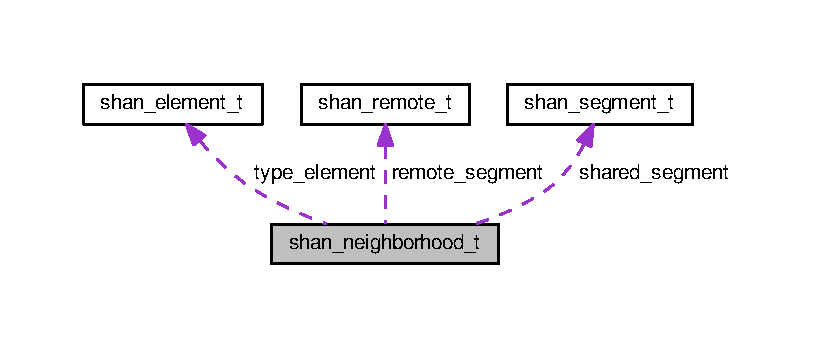
\includegraphics[width=350pt]{structshan__neighborhood__t__coll__graph}
\end{center}
\end{figure}
\subsection*{Public Attributes}
\begin{DoxyCompactItemize}
\item 
int \hyperlink{structshan__neighborhood__t_afaecce1d52b9a980388ca2b90a7433fa}{neighbor\+\_\+hood\+\_\+id}\hypertarget{structshan__neighborhood__t_afaecce1d52b9a980388ca2b90a7433fa}{}\label{structshan__neighborhood__t_afaecce1d52b9a980388ca2b90a7433fa}

\begin{DoxyCompactList}\small\item\em neighborhood id \end{DoxyCompactList}\item 
M\+P\+I\+\_\+\+Comm \hyperlink{structshan__neighborhood__t_af7e2a992b3fb65b9860377d26792ee2d}{M\+P\+I\+\_\+\+C\+O\+M\+M\+\_\+\+S\+HM}\hypertarget{structshan__neighborhood__t_af7e2a992b3fb65b9860377d26792ee2d}{}\label{structshan__neighborhood__t_af7e2a992b3fb65b9860377d26792ee2d}

\begin{DoxyCompactList}\small\item\em shared M\+PI communicator \end{DoxyCompactList}\item 
M\+P\+I\+\_\+\+Comm \hyperlink{structshan__neighborhood__t_a05e33890edbfea469b4190541740c98d}{M\+P\+I\+\_\+\+C\+O\+M\+M\+\_\+\+A\+LL}\hypertarget{structshan__neighborhood__t_a05e33890edbfea469b4190541740c98d}{}\label{structshan__neighborhood__t_a05e33890edbfea469b4190541740c98d}

\begin{DoxyCompactList}\small\item\em global M\+PI communicator \end{DoxyCompactList}\item 
int \hyperlink{structshan__neighborhood__t_a301d36655cb14aa2bce6a47a1ac58653}{num\+\_\+neighbors}\hypertarget{structshan__neighborhood__t_a301d36655cb14aa2bce6a47a1ac58653}{}\label{structshan__neighborhood__t_a301d36655cb14aa2bce6a47a1ac58653}

\begin{DoxyCompactList}\small\item\em num comm partners (neighbors) \end{DoxyCompactList}\item 
int \hyperlink{structshan__neighborhood__t_a220330e5f5b0edb6bdff6b265ea5905f}{num\+\_\+local}\hypertarget{structshan__neighborhood__t_a220330e5f5b0edb6bdff6b265ea5905f}{}\label{structshan__neighborhood__t_a220330e5f5b0edb6bdff6b265ea5905f}

\begin{DoxyCompactList}\small\item\em node local number of comm partners \end{DoxyCompactList}\item 
int $\ast$ \hyperlink{structshan__neighborhood__t_ada9cf12a5dda7681042224a9451134dd}{neighbors}\hypertarget{structshan__neighborhood__t_ada9cf12a5dda7681042224a9451134dd}{}\label{structshan__neighborhood__t_ada9cf12a5dda7681042224a9451134dd}

\begin{DoxyCompactList}\small\item\em list of neighbors, per rank \end{DoxyCompactList}\item 
int $\ast$ \hyperlink{structshan__neighborhood__t_a598f50b99c0c43e6185f2768e6d26d20}{Remote\+Comm\+Index}\hypertarget{structshan__neighborhood__t_a598f50b99c0c43e6185f2768e6d26d20}{}\label{structshan__neighborhood__t_a598f50b99c0c43e6185f2768e6d26d20}

\begin{DoxyCompactList}\small\item\em the remote index corresponding to own rank \end{DoxyCompactList}\item 
int $\ast$ \hyperlink{structshan__neighborhood__t_a7f242a84be34d7098136a4e29e461258}{Remote\+Num\+Neighbors}\hypertarget{structshan__neighborhood__t_a7f242a84be34d7098136a4e29e461258}{}\label{structshan__neighborhood__t_a7f242a84be34d7098136a4e29e461258}

\begin{DoxyCompactList}\small\item\em remote number of neighbors for Remote\+Comm\+Index \end{DoxyCompactList}\item 
int \hyperlink{structshan__neighborhood__t_af69002e058000abbcbebab83632eadff}{num\+\_\+type}\hypertarget{structshan__neighborhood__t_af69002e058000abbcbebab83632eadff}{}\label{structshan__neighborhood__t_af69002e058000abbcbebab83632eadff}

\begin{DoxyCompactList}\small\item\em num types \end{DoxyCompactList}\item 
long $\ast$ \hyperlink{structshan__neighborhood__t_aff6024d0240bae9fcda7c7810706e2cc}{type\+Offset}\hypertarget{structshan__neighborhood__t_aff6024d0240bae9fcda7c7810706e2cc}{}\label{structshan__neighborhood__t_aff6024d0240bae9fcda7c7810706e2cc}

\begin{DoxyCompactList}\small\item\em type offsets for all node local ranks \end{DoxyCompactList}\item 
\hyperlink{structshan__segment__t}{shan\+\_\+segment\+\_\+t} \hyperlink{structshan__neighborhood__t_a6327fe11775d0b3ed3c256865f5cd52c}{shared\+\_\+segment}\hypertarget{structshan__neighborhood__t_a6327fe11775d0b3ed3c256865f5cd52c}{}\label{structshan__neighborhood__t_a6327fe11775d0b3ed3c256865f5cd52c}

\begin{DoxyCompactList}\small\item\em shared window for local communication \end{DoxyCompactList}\item 
\hyperlink{structshan__element__t}{shan\+\_\+element\+\_\+t} $\ast$ \hyperlink{structshan__neighborhood__t_a30a4cb5c30b44753136a36ca493fcf19}{type\+\_\+element}\hypertarget{structshan__neighborhood__t_a30a4cb5c30b44753136a36ca493fcf19}{}\label{structshan__neighborhood__t_a30a4cb5c30b44753136a36ca493fcf19}

\begin{DoxyCompactList}\small\item\em local comm data for remote communication. \end{DoxyCompactList}\item 
long \hyperlink{structshan__neighborhood__t_a4e8665c692837d5851b87fb6d843f71c}{remote\+Sz}\hypertarget{structshan__neighborhood__t_a4e8665c692837d5851b87fb6d843f71c}{}\label{structshan__neighborhood__t_a4e8665c692837d5851b87fb6d843f71c}

\begin{DoxyCompactList}\small\item\em remote comm size, all types, send + recv (byte) \end{DoxyCompactList}\item 
\hyperlink{structshan__remote__t}{shan\+\_\+remote\+\_\+t} \hyperlink{structshan__neighborhood__t_a570ccb16f2652f23e733c69d8bb3022a}{remote\+\_\+segment}\hypertarget{structshan__neighborhood__t_a570ccb16f2652f23e733c69d8bb3022a}{}\label{structshan__neighborhood__t_a570ccb16f2652f23e733c69d8bb3022a}

\begin{DoxyCompactList}\small\item\em private segment for remote communication \end{DoxyCompactList}\item 
int \hyperlink{structshan__neighborhood__t_a4d30862e28f83fda7d13027d65027421}{n\+Proc\+Local}\hypertarget{structshan__neighborhood__t_a4d30862e28f83fda7d13027d65027421}{}\label{structshan__neighborhood__t_a4d30862e28f83fda7d13027d65027421}

\begin{DoxyCompactList}\small\item\em num local ranks in shared mem \end{DoxyCompactList}\item 
int \hyperlink{structshan__neighborhood__t_a47e7148518b93b94c3e8c142c1420991}{i\+Proc\+Local}\hypertarget{structshan__neighborhood__t_a47e7148518b93b94c3e8c142c1420991}{}\label{structshan__neighborhood__t_a47e7148518b93b94c3e8c142c1420991}

\begin{DoxyCompactList}\small\item\em local rank id \end{DoxyCompactList}\item 
int \hyperlink{structshan__neighborhood__t_a4653c428444c2a21348040713122081f}{n\+Proc\+Global}\hypertarget{structshan__neighborhood__t_a4653c428444c2a21348040713122081f}{}\label{structshan__neighborhood__t_a4653c428444c2a21348040713122081f}

\begin{DoxyCompactList}\small\item\em num global ranks \end{DoxyCompactList}\item 
int \hyperlink{structshan__neighborhood__t_abce576cf20a429fd2c9d6385b8cd5949}{i\+Proc\+Global}\hypertarget{structshan__neighborhood__t_abce576cf20a429fd2c9d6385b8cd5949}{}\label{structshan__neighborhood__t_abce576cf20a429fd2c9d6385b8cd5949}

\begin{DoxyCompactList}\small\item\em global rank id \end{DoxyCompactList}\item 
int \hyperlink{structshan__neighborhood__t_a82b099408b246aaec24805ae58f782c6}{master}\hypertarget{structshan__neighborhood__t_a82b099408b246aaec24805ae58f782c6}{}\label{structshan__neighborhood__t_a82b099408b246aaec24805ae58f782c6}

\begin{DoxyCompactList}\small\item\em master of shared segment (local rank 0) \end{DoxyCompactList}\item 
int $\ast$ \hyperlink{structshan__neighborhood__t_add15074f417ea77570915a4b91433122}{remote\+\_\+master}\hypertarget{structshan__neighborhood__t_add15074f417ea77570915a4b91433122}{}\label{structshan__neighborhood__t_add15074f417ea77570915a4b91433122}

\begin{DoxyCompactList}\small\item\em global list of masters \end{DoxyCompactList}\item 
int $\ast$ \hyperlink{structshan__neighborhood__t_a4fabbed69a9715f87876a36a4a88c26a}{local\+\_\+stage\+\_\+count}\hypertarget{structshan__neighborhood__t_a4fabbed69a9715f87876a36a4a88c26a}{}\label{structshan__neighborhood__t_a4fabbed69a9715f87876a36a4a88c26a}

\begin{DoxyCompactList}\small\item\em generic stage counter for wait4\+All(Send/\+Recv) \end{DoxyCompactList}\end{DoxyCompactItemize}


\subsection{Detailed Description}
neighborhood comm struct, holds all communication information for the neighborhood. 

The documentation for this struct was generated from the following file\+:\begin{DoxyCompactItemize}
\item 
include/\hyperlink{SHAN__comm_8h}{S\+H\+A\+N\+\_\+comm.\+h}\end{DoxyCompactItemize}

\hypertarget{structshan__notification__t}{}\section{shan\+\_\+notification\+\_\+t Struct Reference}
\label{structshan__notification__t}\index{shan\+\_\+notification\+\_\+t@{shan\+\_\+notification\+\_\+t}}


{\ttfamily \#include $<$S\+H\+A\+N\+\_\+segment.\+h$>$}

\subsection*{Public Member Functions}
\begin{DoxyCompactItemize}
\item 
volatile int val \hyperlink{structshan__notification__t_a19ff3d7ed20866127745591e3bdd7925}{\+\_\+\+\_\+attribute\+\_\+\+\_\+} ((aligned(64)))\hypertarget{structshan__notification__t_a19ff3d7ed20866127745591e3bdd7925}{}\label{structshan__notification__t_a19ff3d7ed20866127745591e3bdd7925}

\begin{DoxyCompactList}\small\item\em notification value \end{DoxyCompactList}\end{DoxyCompactItemize}


\subsection{Detailed Description}
64 byte aligned notifications struct for shared mem notifications. 

The documentation for this struct was generated from the following file\+:\begin{DoxyCompactItemize}
\item 
include/\hyperlink{SHAN__segment_8h}{S\+H\+A\+N\+\_\+segment.\+h}\end{DoxyCompactItemize}

\hypertarget{structshan__remote__t}{}\section{shan\+\_\+remote\+\_\+t Struct Reference}
\label{structshan__remote__t}\index{shan\+\_\+remote\+\_\+t@{shan\+\_\+remote\+\_\+t}}


{\ttfamily \#include $<$S\+H\+A\+N\+\_\+comm.\+h$>$}

\subsection*{Public Attributes}
\begin{DoxyCompactItemize}
\item 
int \hyperlink{structshan__remote__t_a1b23c142128b38ded6fbeebd87daad3e}{shan\+\_\+id}\hypertarget{structshan__remote__t_a1b23c142128b38ded6fbeebd87daad3e}{}\label{structshan__remote__t_a1b23c142128b38ded6fbeebd87daad3e}

\begin{DoxyCompactList}\small\item\em shared segment id \end{DoxyCompactList}\item 
long \hyperlink{structshan__remote__t_aa70d5714424043c96b0d612b664d985a}{data\+Sz}\hypertarget{structshan__remote__t_aa70d5714424043c96b0d612b664d985a}{}\label{structshan__remote__t_aa70d5714424043c96b0d612b664d985a}

\begin{DoxyCompactList}\small\item\em segment size array \end{DoxyCompactList}\item 
void $\ast$ \hyperlink{structshan__remote__t_aa928d17d58a533646435dcff0435003e}{shan\+\_\+ptr}\hypertarget{structshan__remote__t_aa928d17d58a533646435dcff0435003e}{}\label{structshan__remote__t_aa928d17d58a533646435dcff0435003e}

\begin{DoxyCompactList}\small\item\em local segment pointer \end{DoxyCompactList}\end{DoxyCompactItemize}


\subsection{Detailed Description}
Segment struct, rank\+\_\+local, holds all segment information. 

The documentation for this struct was generated from the following file\+:\begin{DoxyCompactItemize}
\item 
include/\hyperlink{SHAN__comm_8h}{S\+H\+A\+N\+\_\+comm.\+h}\end{DoxyCompactItemize}

\hypertarget{structshan__segment__t}{}\section{shan\+\_\+segment\+\_\+t Struct Reference}
\label{structshan__segment__t}\index{shan\+\_\+segment\+\_\+t@{shan\+\_\+segment\+\_\+t}}


{\ttfamily \#include $<$S\+H\+A\+N\+\_\+segment.\+h$>$}

\subsection*{Public Attributes}
\begin{DoxyCompactItemize}
\item 
void $\ast$$\ast$restrict \hyperlink{structshan__segment__t_a2ec15787570192a7727f626b93b1e3f2}{ptr\+\_\+array}\hypertarget{structshan__segment__t_a2ec15787570192a7727f626b93b1e3f2}{}\label{structshan__segment__t_a2ec15787570192a7727f626b93b1e3f2}

\begin{DoxyCompactList}\small\item\em shan ptr array \end{DoxyCompactList}\item 
int \hyperlink{structshan__segment__t_a7fc2a9c4ec895c92e874d61e9f5bd5f8}{shan\+\_\+id}\hypertarget{structshan__segment__t_a7fc2a9c4ec895c92e874d61e9f5bd5f8}{}\label{structshan__segment__t_a7fc2a9c4ec895c92e874d61e9f5bd5f8}

\begin{DoxyCompactList}\small\item\em shared segment id \end{DoxyCompactList}\item 
int \hyperlink{structshan__segment__t_a4730e781a4ddde44a0d6d60b14abf100}{shan\+\_\+type}\hypertarget{structshan__segment__t_a4730e781a4ddde44a0d6d60b14abf100}{}\label{structshan__segment__t_a4730e781a4ddde44a0d6d60b14abf100}

\begin{DoxyCompactList}\small\item\em shared segment type \end{DoxyCompactList}\item 
long \hyperlink{structshan__segment__t_a55fbd0ba1fdb9e79c43ad9f5d491ee1e}{data\+Sz}\hypertarget{structshan__segment__t_a55fbd0ba1fdb9e79c43ad9f5d491ee1e}{}\label{structshan__segment__t_a55fbd0ba1fdb9e79c43ad9f5d491ee1e}

\begin{DoxyCompactList}\small\item\em segment size \end{DoxyCompactList}\item 
long $\ast$ \hyperlink{structshan__segment__t_a728fe9b7f733a51569a8ede8eebe2771}{local\+Data\+Sz}\hypertarget{structshan__segment__t_a728fe9b7f733a51569a8ede8eebe2771}{}\label{structshan__segment__t_a728fe9b7f733a51569a8ede8eebe2771}

\begin{DoxyCompactList}\small\item\em segment size array \end{DoxyCompactList}\item 
M\+P\+I\+\_\+\+Comm \hyperlink{structshan__segment__t_a0ef0eb1f9f3d377c39b54e847598e2d2}{M\+P\+I\+\_\+\+C\+O\+M\+M\+\_\+\+S\+HM}\hypertarget{structshan__segment__t_a0ef0eb1f9f3d377c39b54e847598e2d2}{}\label{structshan__segment__t_a0ef0eb1f9f3d377c39b54e847598e2d2}

\begin{DoxyCompactList}\small\item\em M\+PI shared mem communicator. \end{DoxyCompactList}\item 
int $\ast$ \hyperlink{structshan__segment__t_a66ac76e179662513f0b6d7fdad6f054d}{fd}\hypertarget{structshan__segment__t_a66ac76e179662513f0b6d7fdad6f054d}{}\label{structshan__segment__t_a66ac76e179662513f0b6d7fdad6f054d}

\begin{DoxyCompactList}\small\item\em shmem file descriptor array \end{DoxyCompactList}\item 
char \hyperlink{structshan__segment__t_aa5f870d8d68479790654e99c8eae5edd}{shan\+\_\+domain\+\_\+name} \mbox{[}80\mbox{]}\hypertarget{structshan__segment__t_aa5f870d8d68479790654e99c8eae5edd}{}\label{structshan__segment__t_aa5f870d8d68479790654e99c8eae5edd}

\begin{DoxyCompactList}\small\item\em unique shmem name \end{DoxyCompactList}\end{DoxyCompactItemize}


\subsection{Detailed Description}
Segment struct, shared, holds all segment information. 

The documentation for this struct was generated from the following file\+:\begin{DoxyCompactItemize}
\item 
include/\hyperlink{SHAN__segment_8h}{S\+H\+A\+N\+\_\+segment.\+h}\end{DoxyCompactItemize}

\hypertarget{structtype__local__t}{}\section{type\+\_\+local\+\_\+t Struct Reference}
\label{structtype__local__t}\index{type\+\_\+local\+\_\+t@{type\+\_\+local\+\_\+t}}


{\ttfamily \#include $<$S\+H\+A\+N\+\_\+comm.\+h$>$}



Collaboration diagram for type\+\_\+local\+\_\+t\+:\nopagebreak
\begin{figure}[H]
\begin{center}
\leavevmode
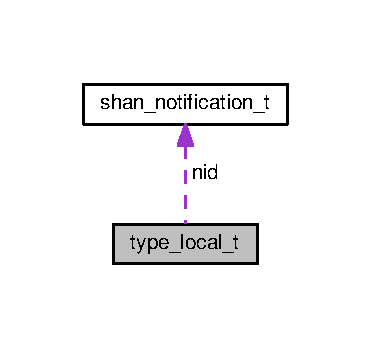
\includegraphics[width=178pt]{structtype__local__t__coll__graph}
\end{center}
\end{figure}
\subsection*{Public Attributes}
\begin{DoxyCompactItemize}
\item 
\hyperlink{structshan__notification__t}{shan\+\_\+notification\+\_\+t} $\ast$ \hyperlink{structtype__local__t_a539eb4f70c6d42aa34d37da44878c250}{nid}\hypertarget{structtype__local__t_a539eb4f70c6d42aa34d37da44878c250}{}\label{structtype__local__t_a539eb4f70c6d42aa34d37da44878c250}

\begin{DoxyCompactList}\small\item\em synchronization for types \end{DoxyCompactList}\item 
int $\ast$ \hyperlink{structtype__local__t_a411a0a1a6eda5686f746f3de1f20c6e3}{nelem\+\_\+send}\hypertarget{structtype__local__t_a411a0a1a6eda5686f746f3de1f20c6e3}{}\label{structtype__local__t_a411a0a1a6eda5686f746f3de1f20c6e3}

\begin{DoxyCompactList}\small\item\em current num send elements per neighbor \end{DoxyCompactList}\item 
int $\ast$ \hyperlink{structtype__local__t_af839d7095a08b4a8345b213b9818f8a8}{nelem\+\_\+recv}\hypertarget{structtype__local__t_af839d7095a08b4a8345b213b9818f8a8}{}\label{structtype__local__t_af839d7095a08b4a8345b213b9818f8a8}

\begin{DoxyCompactList}\small\item\em current num recv elements per neighbor \end{DoxyCompactList}\item 
int $\ast$ \hyperlink{structtype__local__t_ab351d8e498f4f28d06e428b3905ff2d6}{send\+\_\+sz}\hypertarget{structtype__local__t_ab351d8e498f4f28d06e428b3905ff2d6}{}\label{structtype__local__t_ab351d8e498f4f28d06e428b3905ff2d6}

\begin{DoxyCompactList}\small\item\em current send size (in char) per neighbor \end{DoxyCompactList}\item 
int $\ast$ \hyperlink{structtype__local__t_a15d3eb64719efc49430810bcb9fdb307}{recv\+\_\+sz}\hypertarget{structtype__local__t_a15d3eb64719efc49430810bcb9fdb307}{}\label{structtype__local__t_a15d3eb64719efc49430810bcb9fdb307}

\begin{DoxyCompactList}\small\item\em current recv size (in char) per neighbor \end{DoxyCompactList}\item 
long $\ast$ \hyperlink{structtype__local__t_add659698b11598e9b0a36ccd78d01366}{send\+\_\+offset}\hypertarget{structtype__local__t_add659698b11598e9b0a36ccd78d01366}{}\label{structtype__local__t_add659698b11598e9b0a36ccd78d01366}

\begin{DoxyCompactList}\small\item\em list of send offsets per neighbor \end{DoxyCompactList}\item 
long $\ast$ \hyperlink{structtype__local__t_a0b6b2511ba9518d3adfe01807203a6ac}{recv\+\_\+offset}\hypertarget{structtype__local__t_a0b6b2511ba9518d3adfe01807203a6ac}{}\label{structtype__local__t_a0b6b2511ba9518d3adfe01807203a6ac}

\begin{DoxyCompactList}\small\item\em list of recv offsets per neighbor \end{DoxyCompactList}\end{DoxyCompactItemize}


\subsection{Detailed Description}
Type struct, visible in shared memory 

The documentation for this struct was generated from the following file\+:\begin{DoxyCompactItemize}
\item 
include/\hyperlink{SHAN__comm_8h}{S\+H\+A\+N\+\_\+comm.\+h}\end{DoxyCompactItemize}

\chapter{File Documentation}
\hypertarget{F__SHAN_8h}{}\section{include/\+F\+\_\+\+S\+H\+AN.h File Reference}
\label{F__SHAN_8h}\index{include/\+F\+\_\+\+S\+H\+A\+N.\+h@{include/\+F\+\_\+\+S\+H\+A\+N.\+h}}


Wrapper functions for the S\+H\+AN library, mostly targeted at fortran applications.  


{\ttfamily \#include $<$mpi.\+h$>$}\\*
{\ttfamily \#include \char`\"{}S\+H\+A\+N\+\_\+segment.\+h\char`\"{}}\\*
Include dependency graph for F\+\_\+\+S\+H\+A\+N.\+h\+:\nopagebreak
\begin{figure}[H]
\begin{center}
\leavevmode
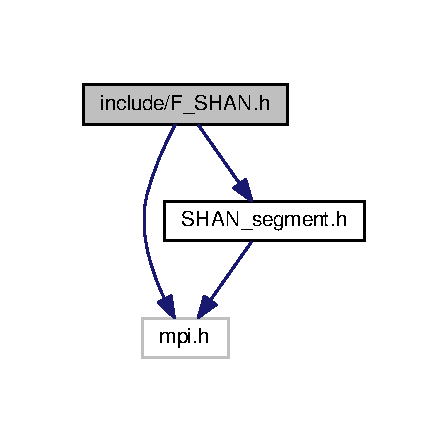
\includegraphics[width=215pt]{F__SHAN_8h__incl}
\end{center}
\end{figure}
\subsection*{Functions}
\begin{DoxyCompactItemize}
\item 
void \hyperlink{F__SHAN_8h_ad0a532af7543afb2885e69f4a924e99f}{f\+\_\+shan\+\_\+alloc\+\_\+shared} (const int segment\+\_\+id, const long data\+Sz, void $\ast$$\ast$restrict shm\+\_\+ptr)
\item 
void \hyperlink{F__SHAN_8h_afffc54aed065493f27f2fc7b9cd7dde8}{f\+\_\+shan\+\_\+free\+\_\+shared} (const int segment\+\_\+id)
\item 
void \hyperlink{F__SHAN_8h_afa13a775a40aa35f9edac001cf922e57}{f\+\_\+shan\+\_\+free\+\_\+comm} (const int neighbor\+\_\+hood\+\_\+id)
\item 
void \hyperlink{F__SHAN_8h_a542d9750aee3a7d14e5325d90a225000}{f\+\_\+shan\+\_\+init\+\_\+comm} (const int neighbor\+\_\+hood\+\_\+id, void $\ast$neighbors, int num\+\_\+neighbors, void $\ast$max\+Send\+Sz, void $\ast$max\+Recv\+Sz, void $\ast$max\+\_\+nelem\+\_\+send, void $\ast$max\+\_\+nelem\+\_\+recv, int num\+\_\+type)
\item 
void \hyperlink{F__SHAN_8h_aa55f47af6341aee177c76705433f0d2d}{f\+\_\+shan\+\_\+type\+\_\+offset} (const int neighbor\+\_\+hood\+\_\+id, const int type\+\_\+id, void $\ast$$\ast$nelem\+\_\+send, void $\ast$$\ast$nelem\+\_\+recv, void $\ast$$\ast$send\+\_\+sz, void $\ast$$\ast$recv\+\_\+sz, void $\ast$$\ast$send\+\_\+idx, void $\ast$$\ast$recv\+\_\+idx)
\item 
void \hyperlink{F__SHAN_8h_a049bea866fe12fd35e9f9f82c0f31d98}{f\+\_\+shan\+\_\+comm\+\_\+wait4\+All} (const int neighbor\+\_\+hood\+\_\+id, const int segment\+\_\+id, const int type\+\_\+id)
\item 
void \hyperlink{F__SHAN_8h_a847423dfe507ddeaf1353932727d0dc3}{f\+\_\+shan\+\_\+comm\+\_\+wait4\+All\+Send} (const int neighbor\+\_\+hood\+\_\+id, const int type\+\_\+id)
\item 
void \hyperlink{F__SHAN_8h_ac5848c5a30bf0996781e1ac23f90352a}{f\+\_\+shan\+\_\+comm\+\_\+wait4\+All\+Recv} (const int neighbor\+\_\+hood\+\_\+id, const int segment\+\_\+id, const int type\+\_\+id)
\item 
void \hyperlink{F__SHAN_8h_aa10d15a629f4514a436a334808043d9c}{f\+\_\+shan\+\_\+comm\+\_\+notify\+\_\+or\+\_\+write} (const int neighbor\+\_\+hood\+\_\+id, const int segment\+\_\+id, const int type\+\_\+id, int idx)
\end{DoxyCompactItemize}


\subsection{Detailed Description}
Wrapper functions for the S\+H\+AN library, mostly targeted at fortran applications. 



\subsection{Function Documentation}
\index{F\+\_\+\+S\+H\+A\+N.\+h@{F\+\_\+\+S\+H\+A\+N.\+h}!f\+\_\+shan\+\_\+alloc\+\_\+shared@{f\+\_\+shan\+\_\+alloc\+\_\+shared}}
\index{f\+\_\+shan\+\_\+alloc\+\_\+shared@{f\+\_\+shan\+\_\+alloc\+\_\+shared}!F\+\_\+\+S\+H\+A\+N.\+h@{F\+\_\+\+S\+H\+A\+N.\+h}}
\subsubsection[{\texorpdfstring{f\+\_\+shan\+\_\+alloc\+\_\+shared(const int segment\+\_\+id, const long data\+Sz, void $\ast$$\ast$restrict shm\+\_\+ptr)}{f_shan_alloc_shared(const int segment_id, const long dataSz, void **restrict shm_ptr)}}]{\setlength{\rightskip}{0pt plus 5cm}void f\+\_\+shan\+\_\+alloc\+\_\+shared (
\begin{DoxyParamCaption}
\item[{const int}]{segment\+\_\+id, }
\item[{const long}]{data\+Sz, }
\item[{void $\ast$$\ast$restrict}]{shm\+\_\+ptr}
\end{DoxyParamCaption}
)}\hypertarget{F__SHAN_8h_ad0a532af7543afb2885e69f4a924e99f}{}\label{F__SHAN_8h_ad0a532af7543afb2885e69f4a924e99f}
wrapper function for shan\+\_\+alloc\+\_\+shared

Note\+: Memory will be page-\/aligned.


\begin{DoxyParams}{Parameters}
{\em segment\+\_\+id} & -\/ segment handle (data) \\
\hline
{\em data\+Sz} & -\/ segment size in byte \\
\hline
{\em shm\+\_\+ptr} & -\/ shared mem pointer for allocated memory\\
\hline
\end{DoxyParams}
\begin{DoxyReturn}{Returns}
S\+H\+A\+N\+\_\+\+S\+U\+C\+C\+E\+SS in case of success, S\+H\+A\+N\+\_\+\+E\+R\+R\+OR in case of error. 
\end{DoxyReturn}
\index{F\+\_\+\+S\+H\+A\+N.\+h@{F\+\_\+\+S\+H\+A\+N.\+h}!f\+\_\+shan\+\_\+comm\+\_\+notify\+\_\+or\+\_\+write@{f\+\_\+shan\+\_\+comm\+\_\+notify\+\_\+or\+\_\+write}}
\index{f\+\_\+shan\+\_\+comm\+\_\+notify\+\_\+or\+\_\+write@{f\+\_\+shan\+\_\+comm\+\_\+notify\+\_\+or\+\_\+write}!F\+\_\+\+S\+H\+A\+N.\+h@{F\+\_\+\+S\+H\+A\+N.\+h}}
\subsubsection[{\texorpdfstring{f\+\_\+shan\+\_\+comm\+\_\+notify\+\_\+or\+\_\+write(const int neighbor\+\_\+hood\+\_\+id, const int segment\+\_\+id, const int type\+\_\+id, int idx)}{f_shan_comm_notify_or_write(const int neighbor_hood_id, const int segment_id, const int type_id, int idx)}}]{\setlength{\rightskip}{0pt plus 5cm}void f\+\_\+shan\+\_\+comm\+\_\+notify\+\_\+or\+\_\+write (
\begin{DoxyParamCaption}
\item[{const int}]{neighbor\+\_\+hood\+\_\+id, }
\item[{const int}]{segment\+\_\+id, }
\item[{const int}]{type\+\_\+id, }
\item[{int}]{idx}
\end{DoxyParamCaption}
)}\hypertarget{F__SHAN_8h_aa10d15a629f4514a436a334808043d9c}{}\label{F__SHAN_8h_aa10d15a629f4514a436a334808043d9c}
wrapper function for shan\+\_\+comm\+\_\+notify\+\_\+or\+\_\+write


\begin{DoxyParams}{Parameters}
{\em neighbor\+\_\+hood\+\_\+id} & -\/ general neighborhood handle \\
\hline
{\em segment\+\_\+id} & -\/ data segment handle \\
\hline
{\em type\+\_\+id} & -\/ used type id \\
\hline
{\em idx} & -\/ comm index for target rank in neighborhood\\
\hline
\end{DoxyParams}
\begin{DoxyReturn}{Returns}
S\+H\+A\+N\+\_\+\+S\+U\+C\+C\+E\+SS in case of success, S\+H\+A\+N\+\_\+\+E\+R\+R\+OR in case of error. 
\end{DoxyReturn}
\index{F\+\_\+\+S\+H\+A\+N.\+h@{F\+\_\+\+S\+H\+A\+N.\+h}!f\+\_\+shan\+\_\+comm\+\_\+wait4\+All@{f\+\_\+shan\+\_\+comm\+\_\+wait4\+All}}
\index{f\+\_\+shan\+\_\+comm\+\_\+wait4\+All@{f\+\_\+shan\+\_\+comm\+\_\+wait4\+All}!F\+\_\+\+S\+H\+A\+N.\+h@{F\+\_\+\+S\+H\+A\+N.\+h}}
\subsubsection[{\texorpdfstring{f\+\_\+shan\+\_\+comm\+\_\+wait4\+All(const int neighbor\+\_\+hood\+\_\+id, const int segment\+\_\+id, const int type\+\_\+id)}{f_shan_comm_wait4All(const int neighbor_hood_id, const int segment_id, const int type_id)}}]{\setlength{\rightskip}{0pt plus 5cm}void f\+\_\+shan\+\_\+comm\+\_\+wait4\+All (
\begin{DoxyParamCaption}
\item[{const int}]{neighbor\+\_\+hood\+\_\+id, }
\item[{const int}]{segment\+\_\+id, }
\item[{const int}]{type\+\_\+id}
\end{DoxyParamCaption}
)}\hypertarget{F__SHAN_8h_a049bea866fe12fd35e9f9f82c0f31d98}{}\label{F__SHAN_8h_a049bea866fe12fd35e9f9f82c0f31d98}
wrapper function for shan\+\_\+comm\+\_\+wait4\+All


\begin{DoxyParams}{Parameters}
{\em neighbor\+\_\+hood\+\_\+id} & -\/ general neighborhood handle \\
\hline
{\em segment\+\_\+id} & -\/ (data) segment handle \\
\hline
{\em type\+\_\+id} & -\/ used type id\\
\hline
\end{DoxyParams}
\begin{DoxyReturn}{Returns}
S\+H\+A\+N\+\_\+\+S\+U\+C\+C\+E\+SS in case of success, S\+H\+A\+N\+\_\+\+E\+R\+R\+OR in case of error. 
\end{DoxyReturn}
\index{F\+\_\+\+S\+H\+A\+N.\+h@{F\+\_\+\+S\+H\+A\+N.\+h}!f\+\_\+shan\+\_\+comm\+\_\+wait4\+All\+Recv@{f\+\_\+shan\+\_\+comm\+\_\+wait4\+All\+Recv}}
\index{f\+\_\+shan\+\_\+comm\+\_\+wait4\+All\+Recv@{f\+\_\+shan\+\_\+comm\+\_\+wait4\+All\+Recv}!F\+\_\+\+S\+H\+A\+N.\+h@{F\+\_\+\+S\+H\+A\+N.\+h}}
\subsubsection[{\texorpdfstring{f\+\_\+shan\+\_\+comm\+\_\+wait4\+All\+Recv(const int neighbor\+\_\+hood\+\_\+id, const int segment\+\_\+id, const int type\+\_\+id)}{f_shan_comm_wait4AllRecv(const int neighbor_hood_id, const int segment_id, const int type_id)}}]{\setlength{\rightskip}{0pt plus 5cm}void f\+\_\+shan\+\_\+comm\+\_\+wait4\+All\+Recv (
\begin{DoxyParamCaption}
\item[{const int}]{neighbor\+\_\+hood\+\_\+id, }
\item[{const int}]{segment\+\_\+id, }
\item[{const int}]{type\+\_\+id}
\end{DoxyParamCaption}
)}\hypertarget{F__SHAN_8h_ac5848c5a30bf0996781e1ac23f90352a}{}\label{F__SHAN_8h_ac5848c5a30bf0996781e1ac23f90352a}
wrapper function for shan\+\_\+comm\+\_\+wait4\+All\+Recv


\begin{DoxyParams}{Parameters}
{\em neighbor\+\_\+hood\+\_\+id} & -\/ general neighborhood handle \\
\hline
{\em segment\+\_\+id} & -\/ (data) segment handle \\
\hline
{\em type\+\_\+id} & -\/ used type id\\
\hline
\end{DoxyParams}
\begin{DoxyReturn}{Returns}
S\+H\+A\+N\+\_\+\+S\+U\+C\+C\+E\+SS in case of success, S\+H\+A\+N\+\_\+\+E\+R\+R\+OR in case of error. 
\end{DoxyReturn}
\index{F\+\_\+\+S\+H\+A\+N.\+h@{F\+\_\+\+S\+H\+A\+N.\+h}!f\+\_\+shan\+\_\+comm\+\_\+wait4\+All\+Send@{f\+\_\+shan\+\_\+comm\+\_\+wait4\+All\+Send}}
\index{f\+\_\+shan\+\_\+comm\+\_\+wait4\+All\+Send@{f\+\_\+shan\+\_\+comm\+\_\+wait4\+All\+Send}!F\+\_\+\+S\+H\+A\+N.\+h@{F\+\_\+\+S\+H\+A\+N.\+h}}
\subsubsection[{\texorpdfstring{f\+\_\+shan\+\_\+comm\+\_\+wait4\+All\+Send(const int neighbor\+\_\+hood\+\_\+id, const int type\+\_\+id)}{f_shan_comm_wait4AllSend(const int neighbor_hood_id, const int type_id)}}]{\setlength{\rightskip}{0pt plus 5cm}void f\+\_\+shan\+\_\+comm\+\_\+wait4\+All\+Send (
\begin{DoxyParamCaption}
\item[{const int}]{neighbor\+\_\+hood\+\_\+id, }
\item[{const int}]{type\+\_\+id}
\end{DoxyParamCaption}
)}\hypertarget{F__SHAN_8h_a847423dfe507ddeaf1353932727d0dc3}{}\label{F__SHAN_8h_a847423dfe507ddeaf1353932727d0dc3}
wrapper function for shan\+\_\+comm\+\_\+wait4\+All\+Send


\begin{DoxyParams}{Parameters}
{\em neighbor\+\_\+hood\+\_\+id} & -\/ general neighborhood handle \\
\hline
{\em type\+\_\+id} & -\/ used type id\\
\hline
\end{DoxyParams}
\begin{DoxyReturn}{Returns}
S\+H\+A\+N\+\_\+\+S\+U\+C\+C\+E\+SS in case of success, S\+H\+A\+N\+\_\+\+E\+R\+R\+OR in case of error. 
\end{DoxyReturn}
\index{F\+\_\+\+S\+H\+A\+N.\+h@{F\+\_\+\+S\+H\+A\+N.\+h}!f\+\_\+shan\+\_\+free\+\_\+comm@{f\+\_\+shan\+\_\+free\+\_\+comm}}
\index{f\+\_\+shan\+\_\+free\+\_\+comm@{f\+\_\+shan\+\_\+free\+\_\+comm}!F\+\_\+\+S\+H\+A\+N.\+h@{F\+\_\+\+S\+H\+A\+N.\+h}}
\subsubsection[{\texorpdfstring{f\+\_\+shan\+\_\+free\+\_\+comm(const int neighbor\+\_\+hood\+\_\+id)}{f_shan_free_comm(const int neighbor_hood_id)}}]{\setlength{\rightskip}{0pt plus 5cm}void f\+\_\+shan\+\_\+free\+\_\+comm (
\begin{DoxyParamCaption}
\item[{const int}]{neighbor\+\_\+hood\+\_\+id}
\end{DoxyParamCaption}
)}\hypertarget{F__SHAN_8h_afa13a775a40aa35f9edac001cf922e57}{}\label{F__SHAN_8h_afa13a775a40aa35f9edac001cf922e57}
wrapper function for shan\+\_\+free\+\_\+comm


\begin{DoxyParams}{Parameters}
{\em neighbor\+\_\+hood\+\_\+id} & -\/ general neighborhood handle\\
\hline
\end{DoxyParams}
\begin{DoxyReturn}{Returns}
S\+H\+A\+N\+\_\+\+S\+U\+C\+C\+E\+SS in case of success, S\+H\+A\+N\+\_\+\+E\+R\+R\+OR in case of error. 
\end{DoxyReturn}
\index{F\+\_\+\+S\+H\+A\+N.\+h@{F\+\_\+\+S\+H\+A\+N.\+h}!f\+\_\+shan\+\_\+free\+\_\+shared@{f\+\_\+shan\+\_\+free\+\_\+shared}}
\index{f\+\_\+shan\+\_\+free\+\_\+shared@{f\+\_\+shan\+\_\+free\+\_\+shared}!F\+\_\+\+S\+H\+A\+N.\+h@{F\+\_\+\+S\+H\+A\+N.\+h}}
\subsubsection[{\texorpdfstring{f\+\_\+shan\+\_\+free\+\_\+shared(const int segment\+\_\+id)}{f_shan_free_shared(const int segment_id)}}]{\setlength{\rightskip}{0pt plus 5cm}void f\+\_\+shan\+\_\+free\+\_\+shared (
\begin{DoxyParamCaption}
\item[{const int}]{segment\+\_\+id}
\end{DoxyParamCaption}
)}\hypertarget{F__SHAN_8h_afffc54aed065493f27f2fc7b9cd7dde8}{}\label{F__SHAN_8h_afffc54aed065493f27f2fc7b9cd7dde8}
wrapper function for shan\+\_\+free\+\_\+shared


\begin{DoxyParams}{Parameters}
{\em segment\+\_\+id} & -\/ segment handle (data)\\
\hline
\end{DoxyParams}
\begin{DoxyReturn}{Returns}
S\+H\+A\+N\+\_\+\+S\+U\+C\+C\+E\+SS in case of success, S\+H\+A\+N\+\_\+\+E\+R\+R\+OR in case of error. 
\end{DoxyReturn}
\index{F\+\_\+\+S\+H\+A\+N.\+h@{F\+\_\+\+S\+H\+A\+N.\+h}!f\+\_\+shan\+\_\+init\+\_\+comm@{f\+\_\+shan\+\_\+init\+\_\+comm}}
\index{f\+\_\+shan\+\_\+init\+\_\+comm@{f\+\_\+shan\+\_\+init\+\_\+comm}!F\+\_\+\+S\+H\+A\+N.\+h@{F\+\_\+\+S\+H\+A\+N.\+h}}
\subsubsection[{\texorpdfstring{f\+\_\+shan\+\_\+init\+\_\+comm(const int neighbor\+\_\+hood\+\_\+id, void $\ast$neighbors, int num\+\_\+neighbors, void $\ast$max\+Send\+Sz, void $\ast$max\+Recv\+Sz, void $\ast$max\+\_\+nelem\+\_\+send, void $\ast$max\+\_\+nelem\+\_\+recv, int num\+\_\+type)}{f_shan_init_comm(const int neighbor_hood_id, void *neighbors, int num_neighbors, void *maxSendSz, void *maxRecvSz, void *max_nelem_send, void *max_nelem_recv, int num_type)}}]{\setlength{\rightskip}{0pt plus 5cm}void f\+\_\+shan\+\_\+init\+\_\+comm (
\begin{DoxyParamCaption}
\item[{const int}]{neighbor\+\_\+hood\+\_\+id, }
\item[{void $\ast$}]{neighbors, }
\item[{int}]{num\+\_\+neighbors, }
\item[{void $\ast$}]{max\+Send\+Sz, }
\item[{void $\ast$}]{max\+Recv\+Sz, }
\item[{void $\ast$}]{max\+\_\+nelem\+\_\+send, }
\item[{void $\ast$}]{max\+\_\+nelem\+\_\+recv, }
\item[{int}]{num\+\_\+type}
\end{DoxyParamCaption}
)}\hypertarget{F__SHAN_8h_a542d9750aee3a7d14e5325d90a225000}{}\label{F__SHAN_8h_a542d9750aee3a7d14e5325d90a225000}
wrapper function for shan\+\_\+init\+\_\+comm


\begin{DoxyParams}{Parameters}
{\em neighbor\+\_\+hood\+\_\+id} & -\/ general neighborhood handle \\
\hline
{\em neighbors} & -\/ comm partners (neighbors) \\
\hline
{\em num\+\_\+neighbors} & -\/ num comm partners (neighbors) \\
\hline
{\em max\+Send\+Sz} & -\/ max send size for every comm type (byte) \\
\hline
{\em max\+Recv\+Sz} & -\/ max recv size for every comm type (byte) \\
\hline
{\em max\+\_\+nelem\+\_\+send} & -\/ max number of send elements for every comm type \\
\hline
{\em max\+\_\+nelem\+\_\+recv} & -\/ max number of recv elements for every comm type \\
\hline
{\em num\+\_\+type} & -\/ number of types\\
\hline
\end{DoxyParams}
\begin{DoxyReturn}{Returns}
S\+H\+A\+N\+\_\+\+S\+U\+C\+C\+E\+SS in case of success, S\+H\+A\+N\+\_\+\+E\+R\+R\+OR in case of error. 
\end{DoxyReturn}
\index{F\+\_\+\+S\+H\+A\+N.\+h@{F\+\_\+\+S\+H\+A\+N.\+h}!f\+\_\+shan\+\_\+type\+\_\+offset@{f\+\_\+shan\+\_\+type\+\_\+offset}}
\index{f\+\_\+shan\+\_\+type\+\_\+offset@{f\+\_\+shan\+\_\+type\+\_\+offset}!F\+\_\+\+S\+H\+A\+N.\+h@{F\+\_\+\+S\+H\+A\+N.\+h}}
\subsubsection[{\texorpdfstring{f\+\_\+shan\+\_\+type\+\_\+offset(const int neighbor\+\_\+hood\+\_\+id, const int type\+\_\+id, void $\ast$$\ast$nelem\+\_\+send, void $\ast$$\ast$nelem\+\_\+recv, void $\ast$$\ast$send\+\_\+sz, void $\ast$$\ast$recv\+\_\+sz, void $\ast$$\ast$send\+\_\+idx, void $\ast$$\ast$recv\+\_\+idx)}{f_shan_type_offset(const int neighbor_hood_id, const int type_id, void **nelem_send, void **nelem_recv, void **send_sz, void **recv_sz, void **send_idx, void **recv_idx)}}]{\setlength{\rightskip}{0pt plus 5cm}void f\+\_\+shan\+\_\+type\+\_\+offset (
\begin{DoxyParamCaption}
\item[{const int}]{neighbor\+\_\+hood\+\_\+id, }
\item[{const int}]{type\+\_\+id, }
\item[{void $\ast$$\ast$}]{nelem\+\_\+send, }
\item[{void $\ast$$\ast$}]{nelem\+\_\+recv, }
\item[{void $\ast$$\ast$}]{send\+\_\+sz, }
\item[{void $\ast$$\ast$}]{recv\+\_\+sz, }
\item[{void $\ast$$\ast$}]{send\+\_\+idx, }
\item[{void $\ast$$\ast$}]{recv\+\_\+idx}
\end{DoxyParamCaption}
)}\hypertarget{F__SHAN_8h_aa55f47af6341aee177c76705433f0d2d}{}\label{F__SHAN_8h_aa55f47af6341aee177c76705433f0d2d}
wrapper function for shan\+\_\+type\+\_\+offset


\begin{DoxyParams}{Parameters}
{\em neighbor\+\_\+hood\+\_\+id} & -\/ general neighborhood handle \\
\hline
{\em type\+\_\+id} & -\/ used type segment \\
\hline
{\em nelem\+\_\+send} & -\/ ptr for current number of send elements. (in shared mem, visible node locally) \\
\hline
{\em nelem\+\_\+recv} & -\/ ptr for current number of recv elements. (in shared mem, visible node locally) \\
\hline
{\em send\+\_\+sz} & -\/ ptr for current send\+\_\+size. (in shared mem, visible node locally) \\
\hline
{\em recv\+\_\+sz} & -\/ ptr for current recv size. (in shared mem, visible node locally) \\
\hline
{\em send\+\_\+idx} & -\/ ptr for current send offset list. (in shared mem, visible node locally) \\
\hline
{\em recv\+\_\+idx} & -\/ ptr for current recv offset list. (in shared mem, visible node locally)\\
\hline
\end{DoxyParams}
\begin{DoxyReturn}{Returns}
S\+H\+A\+N\+\_\+\+S\+U\+C\+C\+E\+SS in case of success, S\+H\+A\+N\+\_\+\+E\+R\+R\+OR in case of error. 
\end{DoxyReturn}

\hypertarget{SHAN__comm_8h}{}\section{include/\+S\+H\+A\+N\+\_\+comm.h File Reference}
\label{SHAN__comm_8h}\index{include/\+S\+H\+A\+N\+\_\+comm.\+h@{include/\+S\+H\+A\+N\+\_\+comm.\+h}}


S\+H\+A\+N\+\_\+comm header for persistant communication in shared memory.  


{\ttfamily \#include $<$stdio.\+h$>$}\\*
{\ttfamily \#include $<$stdlib.\+h$>$}\\*
{\ttfamily \#include \char`\"{}G\+A\+S\+P\+I.\+h\char`\"{}}\\*
{\ttfamily \#include \char`\"{}S\+H\+A\+N\+\_\+segment.\+h\char`\"{}}\\*
Include dependency graph for S\+H\+A\+N\+\_\+comm.\+h\+:\nopagebreak
\begin{figure}[H]
\begin{center}
\leavevmode
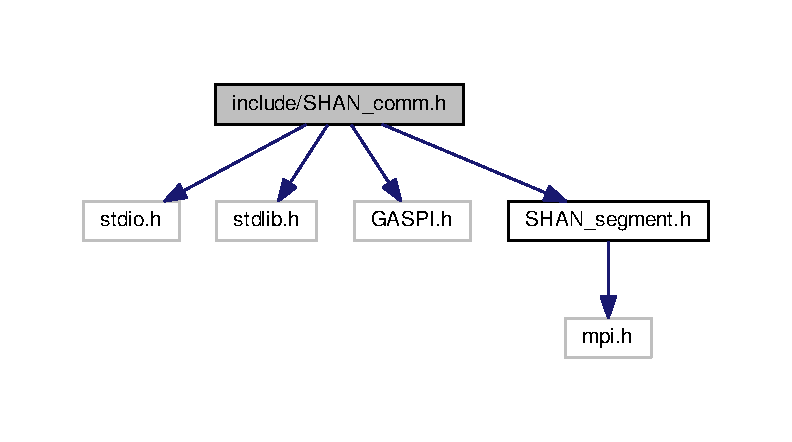
\includegraphics[width=350pt]{SHAN__comm_8h__incl}
\end{center}
\end{figure}
\subsection*{Classes}
\begin{DoxyCompactItemize}
\item 
struct \hyperlink{structtype__local__t}{type\+\_\+local\+\_\+t}
\item 
struct \hyperlink{structshan__remote__t}{shan\+\_\+remote\+\_\+t}
\item 
struct \hyperlink{structshan__element__t}{shan\+\_\+element\+\_\+t}
\item 
struct \hyperlink{structshan__neighborhood__t}{shan\+\_\+neighborhood\+\_\+t}
\end{DoxyCompactItemize}
\subsection*{Macros}
\begin{DoxyCompactItemize}
\item 
\#define \hyperlink{SHAN__comm_8h_a963a5d8c340aca130f096d8f2ccd21d7}{M\+A\+X\+\_\+\+S\+H\+A\+R\+E\+D\+\_\+\+N\+O\+T\+I\+F\+I\+C\+A\+T\+I\+ON}~2\hypertarget{SHAN__comm_8h_a963a5d8c340aca130f096d8f2ccd21d7}{}\label{SHAN__comm_8h_a963a5d8c340aca130f096d8f2ccd21d7}

\begin{DoxyCompactList}\small\item\em \textquotesingle{}have written\textquotesingle{} and \textquotesingle{}have read\textquotesingle{} synchronization \end{DoxyCompactList}\end{DoxyCompactItemize}
\subsection*{Functions}
\begin{DoxyCompactItemize}
\item 
int \hyperlink{SHAN__comm_8h_a680cb28bebeeb0f3292d287fb12fcbcc}{shan\+\_\+comm\+\_\+local\+\_\+rank} (\hyperlink{structshan__neighborhood__t}{shan\+\_\+neighborhood\+\_\+t} $\ast$const neighborhood\+\_\+id, const int rank)
\item 
int \hyperlink{SHAN__comm_8h_a169089b81522332fd280b9c2460bf819}{shan\+\_\+increment\+\_\+local} (\hyperlink{structshan__neighborhood__t}{shan\+\_\+neighborhood\+\_\+t} $\ast$const neighborhood\+\_\+id, int const type\+\_\+id, int const idx)
\item 
int \hyperlink{SHAN__comm_8h_a5d44e5587069a378ea4307dfed59910e}{shan\+\_\+comm\+\_\+init\+\_\+comm} (\hyperlink{structshan__neighborhood__t}{shan\+\_\+neighborhood\+\_\+t} $\ast$const neighborhood\+\_\+id, int neighbor\+\_\+hood\+\_\+id, int $\ast$neighbors, int num\+\_\+neighbors, long $\ast$max\+Send\+Sz, long $\ast$max\+Recv\+Sz, int $\ast$max\+\_\+nelem\+\_\+send, int $\ast$max\+\_\+nelem\+\_\+recv, int num\+\_\+type, M\+P\+I\+\_\+\+Comm M\+P\+I\+\_\+\+C\+O\+M\+M\+\_\+\+S\+HM, M\+P\+I\+\_\+\+Comm M\+P\+I\+\_\+\+C\+O\+M\+M\+\_\+\+A\+LL)
\item 
int \hyperlink{SHAN__comm_8h_a09a54808d1d8919f8b003a25e5a205b8}{shan\+\_\+comm\+\_\+free\+\_\+comm} (\hyperlink{structshan__neighborhood__t}{shan\+\_\+neighborhood\+\_\+t} $\ast$const neighborhood\+\_\+id)
\item 
int \hyperlink{SHAN__comm_8h_aba2ed046030d5a7d7c2af9331d034115}{shan\+\_\+comm\+\_\+notify\+\_\+or\+\_\+write} (\hyperlink{structshan__neighborhood__t}{shan\+\_\+neighborhood\+\_\+t} $\ast$const neighborhood\+\_\+id, \hyperlink{structshan__segment__t}{shan\+\_\+segment\+\_\+t} $\ast$data\+\_\+segment, int type\+\_\+id, int idx)
\item 
int \hyperlink{SHAN__comm_8h_a9cdb53c0ff282a8dad897392c7a7c81c}{shan\+\_\+comm\+\_\+wait4\+All} (\hyperlink{structshan__neighborhood__t}{shan\+\_\+neighborhood\+\_\+t} $\ast$const neighborhood\+\_\+id, \hyperlink{structshan__segment__t}{shan\+\_\+segment\+\_\+t} $\ast$data\+\_\+segment, int type\+\_\+id)
\item 
int \hyperlink{SHAN__comm_8h_a79f1496f7c4af71956e676ac71f4fae2}{shan\+\_\+comm\+\_\+wait4\+All\+Recv} (\hyperlink{structshan__neighborhood__t}{shan\+\_\+neighborhood\+\_\+t} $\ast$const neighborhood\+\_\+id, \hyperlink{structshan__segment__t}{shan\+\_\+segment\+\_\+t} $\ast$data\+\_\+segment, int type\+\_\+id)
\item 
int \hyperlink{SHAN__comm_8h_a5a1c2db2dabfa0d91ca90f6cca1f575a}{shan\+\_\+comm\+\_\+wait4\+Recv} (\hyperlink{structshan__neighborhood__t}{shan\+\_\+neighborhood\+\_\+t} $\ast$const neighborhood\+\_\+id, \hyperlink{structshan__segment__t}{shan\+\_\+segment\+\_\+t} $\ast$data\+\_\+segment, int type\+\_\+id, int idx)
\item 
int \hyperlink{SHAN__comm_8h_a486f4de0ef2600ea95d83f40117884a4}{shan\+\_\+comm\+\_\+test4\+Recv} (\hyperlink{structshan__neighborhood__t}{shan\+\_\+neighborhood\+\_\+t} $\ast$const neighborhood\+\_\+id, \hyperlink{structshan__segment__t}{shan\+\_\+segment\+\_\+t} $\ast$data\+\_\+segment, int type\+\_\+id, int idx)
\item 
int \hyperlink{SHAN__comm_8h_a9a05a500f1218d49846a00a7f8e0145d}{shan\+\_\+comm\+\_\+wait4\+All\+Send} (\hyperlink{structshan__neighborhood__t}{shan\+\_\+neighborhood\+\_\+t} $\ast$const neighborhood\+\_\+id, int type\+\_\+id)
\item 
int \hyperlink{SHAN__comm_8h_acfa6aa7dac777e8357330d1215b71778}{shan\+\_\+comm\+\_\+wait4\+Send} (\hyperlink{structshan__neighborhood__t}{shan\+\_\+neighborhood\+\_\+t} $\ast$const neighborhood\+\_\+id, int type\+\_\+id, int idx)
\item 
int \hyperlink{SHAN__comm_8h_a7c24f1704a2baca4ae43b771caba7e7e}{shan\+\_\+comm\+\_\+test4\+Send} (\hyperlink{structshan__neighborhood__t}{shan\+\_\+neighborhood\+\_\+t} $\ast$const neighborhood\+\_\+id, int type\+\_\+id, int idx)
\item 
void \hyperlink{SHAN__comm_8h_ae7e2ca954282de984bc709f78c34616c}{shan\+\_\+comm\+\_\+shmem\+Barrier} (\hyperlink{structshan__neighborhood__t}{shan\+\_\+neighborhood\+\_\+t} $\ast$const neighborhood\+\_\+id)
\end{DoxyCompactItemize}


\subsection{Detailed Description}
S\+H\+A\+N\+\_\+comm header for persistant communication in shared memory. 



\subsection{Function Documentation}
\index{S\+H\+A\+N\+\_\+comm.\+h@{S\+H\+A\+N\+\_\+comm.\+h}!shan\+\_\+comm\+\_\+free\+\_\+comm@{shan\+\_\+comm\+\_\+free\+\_\+comm}}
\index{shan\+\_\+comm\+\_\+free\+\_\+comm@{shan\+\_\+comm\+\_\+free\+\_\+comm}!S\+H\+A\+N\+\_\+comm.\+h@{S\+H\+A\+N\+\_\+comm.\+h}}
\subsubsection[{\texorpdfstring{shan\+\_\+comm\+\_\+free\+\_\+comm(shan\+\_\+neighborhood\+\_\+t $\ast$const neighborhood\+\_\+id)}{shan_comm_free_comm(shan_neighborhood_t *const neighborhood_id)}}]{\setlength{\rightskip}{0pt plus 5cm}int shan\+\_\+comm\+\_\+free\+\_\+comm (
\begin{DoxyParamCaption}
\item[{{\bf shan\+\_\+neighborhood\+\_\+t} $\ast$const}]{neighborhood\+\_\+id}
\end{DoxyParamCaption}
)}\hypertarget{SHAN__comm_8h_a09a54808d1d8919f8b003a25e5a205b8}{}\label{SHAN__comm_8h_a09a54808d1d8919f8b003a25e5a205b8}
Free communication ressources


\begin{DoxyParams}{Parameters}
{\em neighborhood\+\_\+id} & -\/ general neighborhood handle\\
\hline
\end{DoxyParams}
\begin{DoxyReturn}{Returns}
S\+H\+A\+N\+\_\+\+C\+O\+M\+M\+\_\+\+S\+U\+C\+C\+E\+SS in case of success, S\+H\+A\+N\+\_\+\+C\+O\+M\+M\+\_\+\+E\+R\+R\+OR in case of error. 
\end{DoxyReturn}
\index{S\+H\+A\+N\+\_\+comm.\+h@{S\+H\+A\+N\+\_\+comm.\+h}!shan\+\_\+comm\+\_\+init\+\_\+comm@{shan\+\_\+comm\+\_\+init\+\_\+comm}}
\index{shan\+\_\+comm\+\_\+init\+\_\+comm@{shan\+\_\+comm\+\_\+init\+\_\+comm}!S\+H\+A\+N\+\_\+comm.\+h@{S\+H\+A\+N\+\_\+comm.\+h}}
\subsubsection[{\texorpdfstring{shan\+\_\+comm\+\_\+init\+\_\+comm(shan\+\_\+neighborhood\+\_\+t $\ast$const neighborhood\+\_\+id, int neighbor\+\_\+hood\+\_\+id, int $\ast$neighbors, int num\+\_\+neighbors, long $\ast$max\+Send\+Sz, long $\ast$max\+Recv\+Sz, int $\ast$max\+\_\+nelem\+\_\+send, int $\ast$max\+\_\+nelem\+\_\+recv, int num\+\_\+type, M\+P\+I\+\_\+\+Comm M\+P\+I\+\_\+\+C\+O\+M\+M\+\_\+\+S\+H\+M, M\+P\+I\+\_\+\+Comm M\+P\+I\+\_\+\+C\+O\+M\+M\+\_\+\+A\+L\+L)}{shan_comm_init_comm(shan_neighborhood_t *const neighborhood_id, int neighbor_hood_id, int *neighbors, int num_neighbors, long *maxSendSz, long *maxRecvSz, int *max_nelem_send, int *max_nelem_recv, int num_type, MPI_Comm MPI_COMM_SHM, MPI_Comm MPI_COMM_ALL)}}]{\setlength{\rightskip}{0pt plus 5cm}int shan\+\_\+comm\+\_\+init\+\_\+comm (
\begin{DoxyParamCaption}
\item[{{\bf shan\+\_\+neighborhood\+\_\+t} $\ast$const}]{neighborhood\+\_\+id, }
\item[{int}]{neighbor\+\_\+hood\+\_\+id, }
\item[{int $\ast$}]{neighbors, }
\item[{int}]{num\+\_\+neighbors, }
\item[{long $\ast$}]{max\+Send\+Sz, }
\item[{long $\ast$}]{max\+Recv\+Sz, }
\item[{int $\ast$}]{max\+\_\+nelem\+\_\+send, }
\item[{int $\ast$}]{max\+\_\+nelem\+\_\+recv, }
\item[{int}]{num\+\_\+type, }
\item[{M\+P\+I\+\_\+\+Comm}]{M\+P\+I\+\_\+\+C\+O\+M\+M\+\_\+\+S\+HM, }
\item[{M\+P\+I\+\_\+\+Comm}]{M\+P\+I\+\_\+\+C\+O\+M\+M\+\_\+\+A\+LL}
\end{DoxyParamCaption}
)}\hypertarget{SHAN__comm_8h_a5d44e5587069a378ea4307dfed59910e}{}\label{SHAN__comm_8h_a5d44e5587069a378ea4307dfed59910e}
Initialize persistant communication for shared mem and G\+A\+S\+PI. requires bidirectional communication for synchronization in one-\/sided communication.

A zero length messages will work, no message at all will fail.


\begin{DoxyItemize}
\item allocates shared and private mem for communication (double buffered).
\item figures out local and remote comm partners.
\item negotiates remote number f neighbors and comm index
\end{DoxyItemize}


\begin{DoxyParams}{Parameters}
{\em neighborhood\+\_\+id} & -\/ general neighborhood handle \\
\hline
{\em neighbor\+\_\+hood\+\_\+id} & -\/ neighborhood id \\
\hline
{\em neighbors} & -\/ comm partners (neighbors) \\
\hline
{\em num\+\_\+neighbors} & -\/ num comm partners (neighbors) \\
\hline
{\em max\+Send\+Sz} & -\/ max send size for every type. \\
\hline
{\em max\+Recv\+Sz} & -\/ max recv size for every type \\
\hline
{\em max\+\_\+nelem\+\_\+send} & -\/ max number of send elements per type \\
\hline
{\em max\+\_\+nelem\+\_\+recv} & -\/ max number of recv elements per type \\
\hline
{\em num\+\_\+type} & -\/ number of types \\
\hline
{\em M\+P\+I\+\_\+\+C\+O\+M\+M\+\_\+\+S\+HM} & -\/ M\+PI shared mem communicator \\
\hline
{\em M\+P\+I\+\_\+\+C\+O\+M\+M\+\_\+\+A\+LL} & -\/ embedding of shared communicator (typically M\+P\+I\+\_\+\+C\+O\+M\+M\+\_\+\+W\+O\+R\+LD)\\
\hline
\end{DoxyParams}
\begin{DoxyReturn}{Returns}
S\+H\+A\+N\+\_\+\+C\+O\+M\+M\+\_\+\+S\+U\+C\+C\+E\+SS in case of success, S\+H\+A\+N\+\_\+\+C\+O\+M\+M\+\_\+\+E\+R\+R\+OR in case of error. 
\end{DoxyReturn}
\index{S\+H\+A\+N\+\_\+comm.\+h@{S\+H\+A\+N\+\_\+comm.\+h}!shan\+\_\+comm\+\_\+local\+\_\+rank@{shan\+\_\+comm\+\_\+local\+\_\+rank}}
\index{shan\+\_\+comm\+\_\+local\+\_\+rank@{shan\+\_\+comm\+\_\+local\+\_\+rank}!S\+H\+A\+N\+\_\+comm.\+h@{S\+H\+A\+N\+\_\+comm.\+h}}
\subsubsection[{\texorpdfstring{shan\+\_\+comm\+\_\+local\+\_\+rank(shan\+\_\+neighborhood\+\_\+t $\ast$const neighborhood\+\_\+id, const int rank)}{shan_comm_local_rank(shan_neighborhood_t *const neighborhood_id, const int rank)}}]{\setlength{\rightskip}{0pt plus 5cm}int shan\+\_\+comm\+\_\+local\+\_\+rank (
\begin{DoxyParamCaption}
\item[{{\bf shan\+\_\+neighborhood\+\_\+t} $\ast$const}]{neighborhood\+\_\+id, }
\item[{const int}]{rank}
\end{DoxyParamCaption}
)}\hypertarget{SHAN__comm_8h_a680cb28bebeeb0f3292d287fb12fcbcc}{}\label{SHAN__comm_8h_a680cb28bebeeb0f3292d287fb12fcbcc}
Gets node local rank id.


\begin{DoxyParams}{Parameters}
{\em neighborhood\+\_\+id} & -\/ handle for neighborhood \\
\hline
{\em rank} & -\/ global rank\\
\hline
\end{DoxyParams}
\begin{DoxyReturn}{Returns}
S\+H\+A\+N\+\_\+\+C\+O\+M\+M\+\_\+\+S\+U\+C\+C\+E\+SS in case of success, S\+H\+A\+N\+\_\+\+C\+O\+M\+M\+\_\+\+E\+R\+R\+OR in case of error. 
\end{DoxyReturn}
\index{S\+H\+A\+N\+\_\+comm.\+h@{S\+H\+A\+N\+\_\+comm.\+h}!shan\+\_\+comm\+\_\+notify\+\_\+or\+\_\+write@{shan\+\_\+comm\+\_\+notify\+\_\+or\+\_\+write}}
\index{shan\+\_\+comm\+\_\+notify\+\_\+or\+\_\+write@{shan\+\_\+comm\+\_\+notify\+\_\+or\+\_\+write}!S\+H\+A\+N\+\_\+comm.\+h@{S\+H\+A\+N\+\_\+comm.\+h}}
\subsubsection[{\texorpdfstring{shan\+\_\+comm\+\_\+notify\+\_\+or\+\_\+write(shan\+\_\+neighborhood\+\_\+t $\ast$const neighborhood\+\_\+id, shan\+\_\+segment\+\_\+t $\ast$data\+\_\+segment, int type\+\_\+id, int idx)}{shan_comm_notify_or_write(shan_neighborhood_t *const neighborhood_id, shan_segment_t *data_segment, int type_id, int idx)}}]{\setlength{\rightskip}{0pt plus 5cm}int shan\+\_\+comm\+\_\+notify\+\_\+or\+\_\+write (
\begin{DoxyParamCaption}
\item[{{\bf shan\+\_\+neighborhood\+\_\+t} $\ast$const}]{neighborhood\+\_\+id, }
\item[{{\bf shan\+\_\+segment\+\_\+t} $\ast$}]{data\+\_\+segment, }
\item[{int}]{type\+\_\+id, }
\item[{int}]{idx}
\end{DoxyParamCaption}
)}\hypertarget{SHAN__comm_8h_aba2ed046030d5a7d7c2af9331d034115}{}\label{SHAN__comm_8h_aba2ed046030d5a7d7c2af9331d034115}
Writes data or flags data as readable.


\begin{DoxyItemize}
\item aggregates send data into linear buffer or
\item flags data as readable
\begin{DoxyItemize}
\item number of elements
\item element sizes and
\item element offsets
\end{DoxyItemize}
\end{DoxyItemize}


\begin{DoxyParams}{Parameters}
{\em neighborhood\+\_\+id} & -\/ general neighborhood handle \\
\hline
{\em data\+\_\+segment} & -\/ data segment handle \\
\hline
{\em type\+\_\+id} & -\/ type index \\
\hline
{\em idx} & -\/ comm index for target rank in neighborhood\\
\hline
\end{DoxyParams}
\begin{DoxyReturn}{Returns}
S\+H\+A\+N\+\_\+\+C\+O\+M\+M\+\_\+\+S\+U\+C\+C\+E\+SS in case of success, S\+H\+A\+N\+\_\+\+C\+O\+M\+M\+\_\+\+E\+R\+R\+OR in case of error. 
\end{DoxyReturn}
\index{S\+H\+A\+N\+\_\+comm.\+h@{S\+H\+A\+N\+\_\+comm.\+h}!shan\+\_\+comm\+\_\+shmem\+Barrier@{shan\+\_\+comm\+\_\+shmem\+Barrier}}
\index{shan\+\_\+comm\+\_\+shmem\+Barrier@{shan\+\_\+comm\+\_\+shmem\+Barrier}!S\+H\+A\+N\+\_\+comm.\+h@{S\+H\+A\+N\+\_\+comm.\+h}}
\subsubsection[{\texorpdfstring{shan\+\_\+comm\+\_\+shmem\+Barrier(shan\+\_\+neighborhood\+\_\+t $\ast$const neighborhood\+\_\+id)}{shan_comm_shmemBarrier(shan_neighborhood_t *const neighborhood_id)}}]{\setlength{\rightskip}{0pt plus 5cm}void shan\+\_\+comm\+\_\+shmem\+Barrier (
\begin{DoxyParamCaption}
\item[{{\bf shan\+\_\+neighborhood\+\_\+t} $\ast$const}]{neighborhood\+\_\+id}
\end{DoxyParamCaption}
)}\hypertarget{SHAN__comm_8h_ae7e2ca954282de984bc709f78c34616c}{}\label{SHAN__comm_8h_ae7e2ca954282de984bc709f78c34616c}
Shared mem barrier


\begin{DoxyParams}{Parameters}
{\em neighborhood\+\_\+id} & -\/ general neighborhood handle \\
\hline
\end{DoxyParams}
\index{S\+H\+A\+N\+\_\+comm.\+h@{S\+H\+A\+N\+\_\+comm.\+h}!shan\+\_\+comm\+\_\+test4\+Recv@{shan\+\_\+comm\+\_\+test4\+Recv}}
\index{shan\+\_\+comm\+\_\+test4\+Recv@{shan\+\_\+comm\+\_\+test4\+Recv}!S\+H\+A\+N\+\_\+comm.\+h@{S\+H\+A\+N\+\_\+comm.\+h}}
\subsubsection[{\texorpdfstring{shan\+\_\+comm\+\_\+test4\+Recv(shan\+\_\+neighborhood\+\_\+t $\ast$const neighborhood\+\_\+id, shan\+\_\+segment\+\_\+t $\ast$data\+\_\+segment, int type\+\_\+id, int idx)}{shan_comm_test4Recv(shan_neighborhood_t *const neighborhood_id, shan_segment_t *data_segment, int type_id, int idx)}}]{\setlength{\rightskip}{0pt plus 5cm}int shan\+\_\+comm\+\_\+test4\+Recv (
\begin{DoxyParamCaption}
\item[{{\bf shan\+\_\+neighborhood\+\_\+t} $\ast$const}]{neighborhood\+\_\+id, }
\item[{{\bf shan\+\_\+segment\+\_\+t} $\ast$}]{data\+\_\+segment, }
\item[{int}]{type\+\_\+id, }
\item[{int}]{idx}
\end{DoxyParamCaption}
)}\hypertarget{SHAN__comm_8h_a486f4de0ef2600ea95d83f40117884a4}{}\label{SHAN__comm_8h_a486f4de0ef2600ea95d83f40117884a4}
Tests for specific receive requests.


\begin{DoxyParams}{Parameters}
{\em neighborhood\+\_\+id} & -\/ general neighborhood handle \\
\hline
{\em data\+\_\+segment} & -\/ data segment handle \\
\hline
{\em type\+\_\+id} & -\/ type index \\
\hline
{\em idx} & -\/ comm index for target rank in neighborhood\\
\hline
\end{DoxyParams}
\begin{DoxyReturn}{Returns}
S\+H\+A\+N\+\_\+\+C\+O\+M\+M\+\_\+\+S\+U\+C\+C\+E\+SS in case of success, S\+H\+A\+N\+\_\+\+C\+O\+M\+M\+\_\+\+E\+R\+R\+OR in case of error. 
\end{DoxyReturn}
\index{S\+H\+A\+N\+\_\+comm.\+h@{S\+H\+A\+N\+\_\+comm.\+h}!shan\+\_\+comm\+\_\+test4\+Send@{shan\+\_\+comm\+\_\+test4\+Send}}
\index{shan\+\_\+comm\+\_\+test4\+Send@{shan\+\_\+comm\+\_\+test4\+Send}!S\+H\+A\+N\+\_\+comm.\+h@{S\+H\+A\+N\+\_\+comm.\+h}}
\subsubsection[{\texorpdfstring{shan\+\_\+comm\+\_\+test4\+Send(shan\+\_\+neighborhood\+\_\+t $\ast$const neighborhood\+\_\+id, int type\+\_\+id, int idx)}{shan_comm_test4Send(shan_neighborhood_t *const neighborhood_id, int type_id, int idx)}}]{\setlength{\rightskip}{0pt plus 5cm}int shan\+\_\+comm\+\_\+test4\+Send (
\begin{DoxyParamCaption}
\item[{{\bf shan\+\_\+neighborhood\+\_\+t} $\ast$const}]{neighborhood\+\_\+id, }
\item[{int}]{type\+\_\+id, }
\item[{int}]{idx}
\end{DoxyParamCaption}
)}\hypertarget{SHAN__comm_8h_a7c24f1704a2baca4ae43b771caba7e7e}{}\label{SHAN__comm_8h_a7c24f1704a2baca4ae43b771caba7e7e}
Tests for specific send requests


\begin{DoxyParams}{Parameters}
{\em neighborhood\+\_\+id} & -\/ general neighborhood handle \\
\hline
{\em type\+\_\+id} & -\/ type index \\
\hline
{\em idx} & -\/ comm index for target rank in neighborhood\\
\hline
\end{DoxyParams}
\begin{DoxyReturn}{Returns}
S\+H\+A\+N\+\_\+\+C\+O\+M\+M\+\_\+\+S\+U\+C\+C\+E\+SS in case of success, S\+H\+A\+N\+\_\+\+C\+O\+M\+M\+\_\+\+E\+R\+R\+OR in case of error. 
\end{DoxyReturn}
\index{S\+H\+A\+N\+\_\+comm.\+h@{S\+H\+A\+N\+\_\+comm.\+h}!shan\+\_\+comm\+\_\+wait4\+All@{shan\+\_\+comm\+\_\+wait4\+All}}
\index{shan\+\_\+comm\+\_\+wait4\+All@{shan\+\_\+comm\+\_\+wait4\+All}!S\+H\+A\+N\+\_\+comm.\+h@{S\+H\+A\+N\+\_\+comm.\+h}}
\subsubsection[{\texorpdfstring{shan\+\_\+comm\+\_\+wait4\+All(shan\+\_\+neighborhood\+\_\+t $\ast$const neighborhood\+\_\+id, shan\+\_\+segment\+\_\+t $\ast$data\+\_\+segment, int type\+\_\+id)}{shan_comm_wait4All(shan_neighborhood_t *const neighborhood_id, shan_segment_t *data_segment, int type_id)}}]{\setlength{\rightskip}{0pt plus 5cm}int shan\+\_\+comm\+\_\+wait4\+All (
\begin{DoxyParamCaption}
\item[{{\bf shan\+\_\+neighborhood\+\_\+t} $\ast$const}]{neighborhood\+\_\+id, }
\item[{{\bf shan\+\_\+segment\+\_\+t} $\ast$}]{data\+\_\+segment, }
\item[{int}]{type\+\_\+id}
\end{DoxyParamCaption}
)}\hypertarget{SHAN__comm_8h_a9cdb53c0ff282a8dad897392c7a7c81c}{}\label{SHAN__comm_8h_a9cdb53c0ff282a8dad897392c7a7c81c}
Waits for entire neighborhood


\begin{DoxyItemize}
\item waits for either shared memory notifications or remote G\+A\+S\+PI notifications
\item directly converts send type into recv type in shared memory
\item unpacks pipelined remote communictation into the current receive type.
\item waits for all receive requests.
\item waits for all send requests
\end{DoxyItemize}


\begin{DoxyParams}{Parameters}
{\em neighborhood\+\_\+id} & -\/ general neighborhood handle \\
\hline
{\em data\+\_\+segment} & -\/ data segment handle \\
\hline
{\em type\+\_\+id} & -\/ type index\\
\hline
\end{DoxyParams}
\begin{DoxyReturn}{Returns}
S\+H\+A\+N\+\_\+\+C\+O\+M\+M\+\_\+\+S\+U\+C\+C\+E\+SS in case of success, S\+H\+A\+N\+\_\+\+C\+O\+M\+M\+\_\+\+E\+R\+R\+OR in case of error. 
\end{DoxyReturn}
\index{S\+H\+A\+N\+\_\+comm.\+h@{S\+H\+A\+N\+\_\+comm.\+h}!shan\+\_\+comm\+\_\+wait4\+All\+Recv@{shan\+\_\+comm\+\_\+wait4\+All\+Recv}}
\index{shan\+\_\+comm\+\_\+wait4\+All\+Recv@{shan\+\_\+comm\+\_\+wait4\+All\+Recv}!S\+H\+A\+N\+\_\+comm.\+h@{S\+H\+A\+N\+\_\+comm.\+h}}
\subsubsection[{\texorpdfstring{shan\+\_\+comm\+\_\+wait4\+All\+Recv(shan\+\_\+neighborhood\+\_\+t $\ast$const neighborhood\+\_\+id, shan\+\_\+segment\+\_\+t $\ast$data\+\_\+segment, int type\+\_\+id)}{shan_comm_wait4AllRecv(shan_neighborhood_t *const neighborhood_id, shan_segment_t *data_segment, int type_id)}}]{\setlength{\rightskip}{0pt plus 5cm}int shan\+\_\+comm\+\_\+wait4\+All\+Recv (
\begin{DoxyParamCaption}
\item[{{\bf shan\+\_\+neighborhood\+\_\+t} $\ast$const}]{neighborhood\+\_\+id, }
\item[{{\bf shan\+\_\+segment\+\_\+t} $\ast$}]{data\+\_\+segment, }
\item[{int}]{type\+\_\+id}
\end{DoxyParamCaption}
)}\hypertarget{SHAN__comm_8h_a79f1496f7c4af71956e676ac71f4fae2}{}\label{SHAN__comm_8h_a79f1496f7c4af71956e676ac71f4fae2}
Waits for entire neighborhood


\begin{DoxyItemize}
\item waits for either shared memory notifications or remote G\+A\+S\+PI notifications
\item directly converts send type into recv type in shared memory
\item unpacks pipelined remote communictation into the current receive type.
\item waits for all receive requests.
\end{DoxyItemize}


\begin{DoxyParams}{Parameters}
{\em neighborhood\+\_\+id} & -\/ general neighborhood handle \\
\hline
{\em data\+\_\+segment} & -\/ data segment handle \\
\hline
{\em type\+\_\+id} & -\/ type index\\
\hline
\end{DoxyParams}
\begin{DoxyReturn}{Returns}
S\+H\+A\+N\+\_\+\+C\+O\+M\+M\+\_\+\+S\+U\+C\+C\+E\+SS in case of success, S\+H\+A\+N\+\_\+\+C\+O\+M\+M\+\_\+\+E\+R\+R\+OR in case of error. 
\end{DoxyReturn}
\index{S\+H\+A\+N\+\_\+comm.\+h@{S\+H\+A\+N\+\_\+comm.\+h}!shan\+\_\+comm\+\_\+wait4\+All\+Send@{shan\+\_\+comm\+\_\+wait4\+All\+Send}}
\index{shan\+\_\+comm\+\_\+wait4\+All\+Send@{shan\+\_\+comm\+\_\+wait4\+All\+Send}!S\+H\+A\+N\+\_\+comm.\+h@{S\+H\+A\+N\+\_\+comm.\+h}}
\subsubsection[{\texorpdfstring{shan\+\_\+comm\+\_\+wait4\+All\+Send(shan\+\_\+neighborhood\+\_\+t $\ast$const neighborhood\+\_\+id, int type\+\_\+id)}{shan_comm_wait4AllSend(shan_neighborhood_t *const neighborhood_id, int type_id)}}]{\setlength{\rightskip}{0pt plus 5cm}int shan\+\_\+comm\+\_\+wait4\+All\+Send (
\begin{DoxyParamCaption}
\item[{{\bf shan\+\_\+neighborhood\+\_\+t} $\ast$const}]{neighborhood\+\_\+id, }
\item[{int}]{type\+\_\+id}
\end{DoxyParamCaption}
)}\hypertarget{SHAN__comm_8h_a9a05a500f1218d49846a00a7f8e0145d}{}\label{SHAN__comm_8h_a9a05a500f1218d49846a00a7f8e0145d}
Waits for entire neighborhood


\begin{DoxyItemize}
\item waits for all send requests
\end{DoxyItemize}


\begin{DoxyParams}{Parameters}
{\em neighborhood\+\_\+id} & -\/ general neighborhood handle \\
\hline
{\em type\+\_\+id} & -\/ type index\\
\hline
\end{DoxyParams}
\begin{DoxyReturn}{Returns}
S\+H\+A\+N\+\_\+\+C\+O\+M\+M\+\_\+\+S\+U\+C\+C\+E\+SS in case of success, S\+H\+A\+N\+\_\+\+C\+O\+M\+M\+\_\+\+E\+R\+R\+OR in case of error. 
\end{DoxyReturn}
\index{S\+H\+A\+N\+\_\+comm.\+h@{S\+H\+A\+N\+\_\+comm.\+h}!shan\+\_\+comm\+\_\+wait4\+Recv@{shan\+\_\+comm\+\_\+wait4\+Recv}}
\index{shan\+\_\+comm\+\_\+wait4\+Recv@{shan\+\_\+comm\+\_\+wait4\+Recv}!S\+H\+A\+N\+\_\+comm.\+h@{S\+H\+A\+N\+\_\+comm.\+h}}
\subsubsection[{\texorpdfstring{shan\+\_\+comm\+\_\+wait4\+Recv(shan\+\_\+neighborhood\+\_\+t $\ast$const neighborhood\+\_\+id, shan\+\_\+segment\+\_\+t $\ast$data\+\_\+segment, int type\+\_\+id, int idx)}{shan_comm_wait4Recv(shan_neighborhood_t *const neighborhood_id, shan_segment_t *data_segment, int type_id, int idx)}}]{\setlength{\rightskip}{0pt plus 5cm}int shan\+\_\+comm\+\_\+wait4\+Recv (
\begin{DoxyParamCaption}
\item[{{\bf shan\+\_\+neighborhood\+\_\+t} $\ast$const}]{neighborhood\+\_\+id, }
\item[{{\bf shan\+\_\+segment\+\_\+t} $\ast$}]{data\+\_\+segment, }
\item[{int}]{type\+\_\+id, }
\item[{int}]{idx}
\end{DoxyParamCaption}
)}\hypertarget{SHAN__comm_8h_a5a1c2db2dabfa0d91ca90f6cca1f575a}{}\label{SHAN__comm_8h_a5a1c2db2dabfa0d91ca90f6cca1f575a}
waits for specific receive requests.


\begin{DoxyParams}{Parameters}
{\em neighborhood\+\_\+id} & -\/ general neighborhood handle \\
\hline
{\em data\+\_\+segment} & -\/ data segment handle \\
\hline
{\em type\+\_\+id} & -\/ type index \\
\hline
{\em idx} & -\/ comm index for target rank in neighborhood\\
\hline
\end{DoxyParams}
\begin{DoxyReturn}{Returns}
S\+H\+A\+N\+\_\+\+C\+O\+M\+M\+\_\+\+S\+U\+C\+C\+E\+SS in case of success, S\+H\+A\+N\+\_\+\+C\+O\+M\+M\+\_\+\+E\+R\+R\+OR in case of error. 
\end{DoxyReturn}
\index{S\+H\+A\+N\+\_\+comm.\+h@{S\+H\+A\+N\+\_\+comm.\+h}!shan\+\_\+comm\+\_\+wait4\+Send@{shan\+\_\+comm\+\_\+wait4\+Send}}
\index{shan\+\_\+comm\+\_\+wait4\+Send@{shan\+\_\+comm\+\_\+wait4\+Send}!S\+H\+A\+N\+\_\+comm.\+h@{S\+H\+A\+N\+\_\+comm.\+h}}
\subsubsection[{\texorpdfstring{shan\+\_\+comm\+\_\+wait4\+Send(shan\+\_\+neighborhood\+\_\+t $\ast$const neighborhood\+\_\+id, int type\+\_\+id, int idx)}{shan_comm_wait4Send(shan_neighborhood_t *const neighborhood_id, int type_id, int idx)}}]{\setlength{\rightskip}{0pt plus 5cm}int shan\+\_\+comm\+\_\+wait4\+Send (
\begin{DoxyParamCaption}
\item[{{\bf shan\+\_\+neighborhood\+\_\+t} $\ast$const}]{neighborhood\+\_\+id, }
\item[{int}]{type\+\_\+id, }
\item[{int}]{idx}
\end{DoxyParamCaption}
)}\hypertarget{SHAN__comm_8h_acfa6aa7dac777e8357330d1215b71778}{}\label{SHAN__comm_8h_acfa6aa7dac777e8357330d1215b71778}
Waits for specific send requests


\begin{DoxyParams}{Parameters}
{\em neighborhood\+\_\+id} & -\/ general neighborhood handle \\
\hline
{\em type\+\_\+id} & -\/ type index \\
\hline
{\em idx} & -\/ comm index for target rank in neighborhood\\
\hline
\end{DoxyParams}
\begin{DoxyReturn}{Returns}
S\+H\+A\+N\+\_\+\+C\+O\+M\+M\+\_\+\+S\+U\+C\+C\+E\+SS in case of success, S\+H\+A\+N\+\_\+\+C\+O\+M\+M\+\_\+\+E\+R\+R\+OR in case of error. 
\end{DoxyReturn}
\index{S\+H\+A\+N\+\_\+comm.\+h@{S\+H\+A\+N\+\_\+comm.\+h}!shan\+\_\+increment\+\_\+local@{shan\+\_\+increment\+\_\+local}}
\index{shan\+\_\+increment\+\_\+local@{shan\+\_\+increment\+\_\+local}!S\+H\+A\+N\+\_\+comm.\+h@{S\+H\+A\+N\+\_\+comm.\+h}}
\subsubsection[{\texorpdfstring{shan\+\_\+increment\+\_\+local(shan\+\_\+neighborhood\+\_\+t $\ast$const neighborhood\+\_\+id, int const type\+\_\+id, int const idx)}{shan_increment_local(shan_neighborhood_t *const neighborhood_id, int const type_id, int const idx)}}]{\setlength{\rightskip}{0pt plus 5cm}int shan\+\_\+increment\+\_\+local (
\begin{DoxyParamCaption}
\item[{{\bf shan\+\_\+neighborhood\+\_\+t} $\ast$const}]{neighborhood\+\_\+id, }
\item[{int const}]{type\+\_\+id, }
\item[{int const}]{idx}
\end{DoxyParamCaption}
)}\hypertarget{SHAN__comm_8h_a169089b81522332fd280b9c2460bf819}{}\label{SHAN__comm_8h_a169089b81522332fd280b9c2460bf819}
Increments counter in shared mem


\begin{DoxyParams}{Parameters}
{\em neighborhood\+\_\+id} & -\/ general neighborhood handle \\
\hline
{\em type\+\_\+id} & -\/ type index \\
\hline
{\em idx} & -\/ comm index for target rank in neighborhood\\
\hline
\end{DoxyParams}
\begin{DoxyReturn}{Returns}
S\+H\+A\+N\+\_\+\+C\+O\+M\+M\+\_\+\+S\+U\+C\+C\+E\+SS in case of success, S\+H\+A\+N\+\_\+\+C\+O\+M\+M\+\_\+\+E\+R\+R\+OR in case of error. 
\end{DoxyReturn}

\hypertarget{SHAN__segment_8h}{}\section{include/\+S\+H\+A\+N\+\_\+segment.h File Reference}
\label{SHAN__segment_8h}\index{include/\+S\+H\+A\+N\+\_\+segment.\+h@{include/\+S\+H\+A\+N\+\_\+segment.\+h}}


S\+H\+A\+N\+\_\+segment header for notifications in shared memory.  


{\ttfamily \#include $<$mpi.\+h$>$}\\*
Include dependency graph for S\+H\+A\+N\+\_\+segment.\+h\+:\nopagebreak
\begin{figure}[H]
\begin{center}
\leavevmode
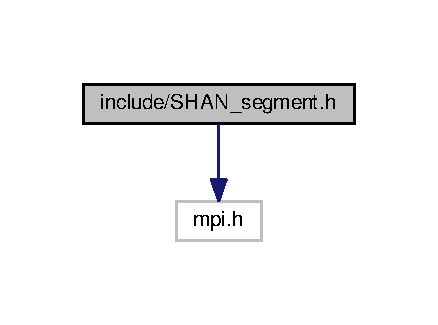
\includegraphics[width=210pt]{SHAN__segment_8h__incl}
\end{center}
\end{figure}
This graph shows which files directly or indirectly include this file\+:\nopagebreak
\begin{figure}[H]
\begin{center}
\leavevmode
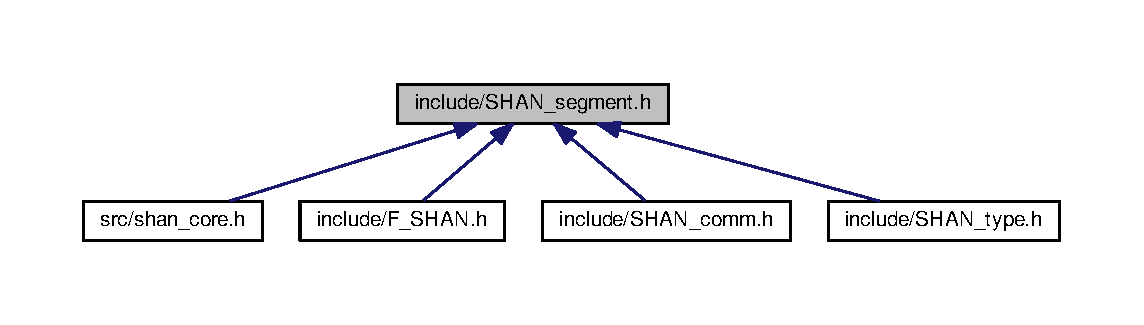
\includegraphics[width=350pt]{SHAN__segment_8h__dep__incl}
\end{center}
\end{figure}
\subsection*{Classes}
\begin{DoxyCompactItemize}
\item 
struct \hyperlink{structshan__notification__t}{shan\+\_\+notification\+\_\+t}
\item 
struct \hyperlink{structshan__segment__t}{shan\+\_\+segment\+\_\+t}
\end{DoxyCompactItemize}
\subsection*{Enumerations}
\begin{DoxyCompactItemize}
\item 
enum {\bfseries shan\+\_\+type} \{ {\bfseries S\+H\+A\+N\+\_\+\+D\+A\+TA} = 0, 
{\bfseries S\+H\+A\+N\+\_\+\+T\+Y\+PE} = 1
 \}\hypertarget{SHAN__segment_8h_abe976d0a720ecb25d9342ca38c2ad206}{}\label{SHAN__segment_8h_abe976d0a720ecb25d9342ca38c2ad206}

\item 
enum {\bfseries shan\+\_\+return\+\_\+val} \{ {\bfseries S\+H\+A\+N\+\_\+\+E\+R\+R\+OR} = -\/2, 
{\bfseries S\+H\+A\+N\+\_\+\+F\+A\+IL} = -\/1, 
{\bfseries S\+H\+A\+N\+\_\+\+S\+U\+C\+C\+E\+SS} = 0
 \}\hypertarget{SHAN__segment_8h_a4690c63731c30ab1590c4e0f527526d2}{}\label{SHAN__segment_8h_a4690c63731c30ab1590c4e0f527526d2}

\end{DoxyCompactItemize}
\subsection*{Functions}
\begin{DoxyCompactItemize}
\item 
int \hyperlink{SHAN__segment_8h_aa45eee114648cecfe8d17e6e3f9c225b}{shan\+\_\+alloc\+\_\+shared} (\hyperlink{structshan__segment__t}{shan\+\_\+segment\+\_\+t} $\ast$const segment, const int shan\+\_\+id, const int shan\+\_\+type, const long data\+Sz, const M\+P\+I\+\_\+\+Comm M\+P\+I\+\_\+\+C\+O\+M\+M\+\_\+\+S\+HM)
\item 
int \hyperlink{SHAN__segment_8h_a149299eae702b7dd00dc5202d0fd177b}{shan\+\_\+free\+\_\+shared} (\hyperlink{structshan__segment__t}{shan\+\_\+segment\+\_\+t} $\ast$const segment)
\item 
int \hyperlink{SHAN__segment_8h_ac38c381b88611d910071682226d80106}{shan\+\_\+get\+\_\+shared\+\_\+ptr} (\hyperlink{structshan__segment__t}{shan\+\_\+segment\+\_\+t} $\ast$const segment, const int rank, void $\ast$$\ast$shm\+\_\+ptr)
\item 
int \hyperlink{SHAN__segment_8h_a0d0ee047fe4462c73a6312e039d34970}{shan\+\_\+notify\+\_\+reset\+\_\+shared} (\hyperlink{structshan__notification__t}{shan\+\_\+notification\+\_\+t} $\ast$const ptr, const int idx, int $\ast$const val)
\item 
int \hyperlink{SHAN__segment_8h_a80250638151a878ad4595dbac46b0232}{shan\+\_\+notify\+\_\+increment\+\_\+shared} (\hyperlink{structshan__notification__t}{shan\+\_\+notification\+\_\+t} $\ast$const ptr, const int idx, const int increment)
\item 
int \hyperlink{SHAN__segment_8h_a0aaa2901cb622fbf2f12145418656aa9}{shan\+\_\+notify\+\_\+test\+\_\+shared} (\hyperlink{structshan__notification__t}{shan\+\_\+notification\+\_\+t} $\ast$const ptr, const int idx, int $\ast$const val)
\item 
int \hyperlink{SHAN__segment_8h_a7686b269f38366738e142f0fc984ea06}{shan\+\_\+notify\+\_\+init\+\_\+shared} (\hyperlink{structshan__notification__t}{shan\+\_\+notification\+\_\+t} $\ast$const ptr, const int idx)
\end{DoxyCompactItemize}


\subsection{Detailed Description}
S\+H\+A\+N\+\_\+segment header for notifications in shared memory. 

The S\+H\+AN (S\+H\+A\+\_\+red N\+\_\+otifications) interface is a user-\/level A\+PI which aims at migrating flat M\+PI (legacy) code towards an asynchronous dataflow model. S\+H\+AN uses the G\+A\+S\+PI A\+PI and extends ideas from M\+PI shared windows.

G\+A\+S\+PI is a P\+G\+AS communication library which is based on the concept of one-\/sided, notified communication. The synchronization context here is bundled together with a one-\/sided message such that a communication target becomes able to test for completion of the received one-\/sided communication.

Traditionally the G\+A\+S\+PI programming model has been aimed at multithreaded or task-\/based applications. In G\+A\+S\+PI the synchronization context is bundled together with a one-\/sided message such that a communication target becomes able to test for completion of the received one-\/sided communication.

In order to support a migration of legacy applications (with a flat M\+PI communication model) towards G\+A\+S\+PI, we have extended the concept of shared M\+PI windows towards a notified communication model in which the processes sharing a common window become able to see all one-\/sided and notified communication targeted at this window. Similarly we have extended the concept of M\+PI shared windows with shared notifications, which are globally visible in shared memory.

Besides the possibility to entirely avoid node-\/internal communication and to make use of a much improved overlap of communication and computation the model of notified communication in G\+A\+S\+PI shared windows will allow legacy S\+P\+MD applications a transition towards an asynchronous dataflow model. 

\subsection{Function Documentation}
\index{S\+H\+A\+N\+\_\+segment.\+h@{S\+H\+A\+N\+\_\+segment.\+h}!shan\+\_\+alloc\+\_\+shared@{shan\+\_\+alloc\+\_\+shared}}
\index{shan\+\_\+alloc\+\_\+shared@{shan\+\_\+alloc\+\_\+shared}!S\+H\+A\+N\+\_\+segment.\+h@{S\+H\+A\+N\+\_\+segment.\+h}}
\subsubsection[{\texorpdfstring{shan\+\_\+alloc\+\_\+shared(shan\+\_\+segment\+\_\+t $\ast$const segment, const int shan\+\_\+id, const int shan\+\_\+type, const long data\+Sz, const M\+P\+I\+\_\+\+Comm M\+P\+I\+\_\+\+C\+O\+M\+M\+\_\+\+S\+H\+M)}{shan_alloc_shared(shan_segment_t *const segment, const int shan_id, const int shan_type, const long dataSz, const MPI_Comm MPI_COMM_SHM)}}]{\setlength{\rightskip}{0pt plus 5cm}int shan\+\_\+alloc\+\_\+shared (
\begin{DoxyParamCaption}
\item[{{\bf shan\+\_\+segment\+\_\+t} $\ast$const}]{segment, }
\item[{const int}]{shan\+\_\+id, }
\item[{const int}]{shan\+\_\+type, }
\item[{const long}]{data\+Sz, }
\item[{const M\+P\+I\+\_\+\+Comm}]{M\+P\+I\+\_\+\+C\+O\+M\+M\+\_\+\+S\+HM}
\end{DoxyParamCaption}
)}\hypertarget{SHAN__segment_8h_aa45eee114648cecfe8d17e6e3f9c225b}{}\label{SHAN__segment_8h_aa45eee114648cecfe8d17e6e3f9c225b}
Local allocation of shared memory of size data\+Sz

Note\+: Memory will be page-\/aligned.


\begin{DoxyParams}{Parameters}
{\em segment} & -\/ segment handle \\
\hline
{\em shan\+\_\+id} & -\/ (unique) segment id \\
\hline
{\em shan\+\_\+type} & -\/ type of allocated memory \\
\hline
{\em data\+Sz} & -\/ required memory size per rank in byte \\
\hline
{\em M\+P\+I\+\_\+\+C\+O\+M\+M\+\_\+\+S\+HM} & -\/ shared mem communicator\\
\hline
\end{DoxyParams}
\begin{DoxyReturn}{Returns}
S\+H\+A\+N\+\_\+\+S\+U\+C\+C\+E\+SS in case of success, S\+H\+A\+N\+\_\+\+E\+R\+R\+OR in case of error. 
\end{DoxyReturn}
\index{S\+H\+A\+N\+\_\+segment.\+h@{S\+H\+A\+N\+\_\+segment.\+h}!shan\+\_\+free\+\_\+shared@{shan\+\_\+free\+\_\+shared}}
\index{shan\+\_\+free\+\_\+shared@{shan\+\_\+free\+\_\+shared}!S\+H\+A\+N\+\_\+segment.\+h@{S\+H\+A\+N\+\_\+segment.\+h}}
\subsubsection[{\texorpdfstring{shan\+\_\+free\+\_\+shared(shan\+\_\+segment\+\_\+t $\ast$const segment)}{shan_free_shared(shan_segment_t *const segment)}}]{\setlength{\rightskip}{0pt plus 5cm}int shan\+\_\+free\+\_\+shared (
\begin{DoxyParamCaption}
\item[{{\bf shan\+\_\+segment\+\_\+t} $\ast$const}]{segment}
\end{DoxyParamCaption}
)}\hypertarget{SHAN__segment_8h_a149299eae702b7dd00dc5202d0fd177b}{}\label{SHAN__segment_8h_a149299eae702b7dd00dc5202d0fd177b}
Free shared memory.


\begin{DoxyParams}{Parameters}
{\em segment} & -\/ segment handle\\
\hline
\end{DoxyParams}
\begin{DoxyReturn}{Returns}
S\+H\+A\+N\+\_\+\+S\+U\+C\+C\+E\+SS in case of success, S\+H\+A\+N\+\_\+\+E\+R\+R\+OR in case of error. 
\end{DoxyReturn}
\index{S\+H\+A\+N\+\_\+segment.\+h@{S\+H\+A\+N\+\_\+segment.\+h}!shan\+\_\+get\+\_\+shared\+\_\+ptr@{shan\+\_\+get\+\_\+shared\+\_\+ptr}}
\index{shan\+\_\+get\+\_\+shared\+\_\+ptr@{shan\+\_\+get\+\_\+shared\+\_\+ptr}!S\+H\+A\+N\+\_\+segment.\+h@{S\+H\+A\+N\+\_\+segment.\+h}}
\subsubsection[{\texorpdfstring{shan\+\_\+get\+\_\+shared\+\_\+ptr(shan\+\_\+segment\+\_\+t $\ast$const segment, const int rank, void $\ast$$\ast$shm\+\_\+ptr)}{shan_get_shared_ptr(shan_segment_t *const segment, const int rank, void **shm_ptr)}}]{\setlength{\rightskip}{0pt plus 5cm}int shan\+\_\+get\+\_\+shared\+\_\+ptr (
\begin{DoxyParamCaption}
\item[{{\bf shan\+\_\+segment\+\_\+t} $\ast$const}]{segment, }
\item[{const int}]{rank, }
\item[{void $\ast$$\ast$}]{shm\+\_\+ptr}
\end{DoxyParamCaption}
)}\hypertarget{SHAN__segment_8h_ac38c381b88611d910071682226d80106}{}\label{SHAN__segment_8h_ac38c381b88611d910071682226d80106}
Gets shared mem pointer for node local ranks


\begin{DoxyParams}{Parameters}
{\em segment} & -\/ segment handle \\
\hline
{\em rank} & -\/ node local rank id \\
\hline
{\em shm\+\_\+ptr} & -\/ required memory size per rank in byte\\
\hline
\end{DoxyParams}
\begin{DoxyReturn}{Returns}
S\+H\+A\+N\+\_\+\+S\+U\+C\+C\+E\+SS in case of success, S\+H\+A\+N\+\_\+\+E\+R\+R\+OR in case of error. 
\end{DoxyReturn}
\index{S\+H\+A\+N\+\_\+segment.\+h@{S\+H\+A\+N\+\_\+segment.\+h}!shan\+\_\+notify\+\_\+increment\+\_\+shared@{shan\+\_\+notify\+\_\+increment\+\_\+shared}}
\index{shan\+\_\+notify\+\_\+increment\+\_\+shared@{shan\+\_\+notify\+\_\+increment\+\_\+shared}!S\+H\+A\+N\+\_\+segment.\+h@{S\+H\+A\+N\+\_\+segment.\+h}}
\subsubsection[{\texorpdfstring{shan\+\_\+notify\+\_\+increment\+\_\+shared(shan\+\_\+notification\+\_\+t $\ast$const ptr, const int idx, const int increment)}{shan_notify_increment_shared(shan_notification_t *const ptr, const int idx, const int increment)}}]{\setlength{\rightskip}{0pt plus 5cm}int shan\+\_\+notify\+\_\+increment\+\_\+shared (
\begin{DoxyParamCaption}
\item[{{\bf shan\+\_\+notification\+\_\+t} $\ast$const}]{ptr, }
\item[{const int}]{idx, }
\item[{const int}]{increment}
\end{DoxyParamCaption}
)}\hypertarget{SHAN__segment_8h_a80250638151a878ad4595dbac46b0232}{}\label{SHAN__segment_8h_a80250638151a878ad4595dbac46b0232}
Increments shared mem notfication. Sets write fence such that local result is valid, once the incremented value is visible for other local ranks.


\begin{DoxyParams}{Parameters}
{\em ptr} & -\/ pointer to shared notification array \\
\hline
{\em idx} & -\/ shared mem notification id \\
\hline
{\em increment} & -\/ increment value\\
\hline
\end{DoxyParams}
\begin{DoxyReturn}{Returns}
S\+H\+A\+N\+\_\+\+S\+U\+C\+C\+E\+SS in case of success, S\+H\+A\+N\+\_\+\+E\+R\+R\+OR in case of error. 
\end{DoxyReturn}
\index{S\+H\+A\+N\+\_\+segment.\+h@{S\+H\+A\+N\+\_\+segment.\+h}!shan\+\_\+notify\+\_\+init\+\_\+shared@{shan\+\_\+notify\+\_\+init\+\_\+shared}}
\index{shan\+\_\+notify\+\_\+init\+\_\+shared@{shan\+\_\+notify\+\_\+init\+\_\+shared}!S\+H\+A\+N\+\_\+segment.\+h@{S\+H\+A\+N\+\_\+segment.\+h}}
\subsubsection[{\texorpdfstring{shan\+\_\+notify\+\_\+init\+\_\+shared(shan\+\_\+notification\+\_\+t $\ast$const ptr, const int idx)}{shan_notify_init_shared(shan_notification_t *const ptr, const int idx)}}]{\setlength{\rightskip}{0pt plus 5cm}int shan\+\_\+notify\+\_\+init\+\_\+shared (
\begin{DoxyParamCaption}
\item[{{\bf shan\+\_\+notification\+\_\+t} $\ast$const}]{ptr, }
\item[{const int}]{idx}
\end{DoxyParamCaption}
)}\hypertarget{SHAN__segment_8h_a7686b269f38366738e142f0fc984ea06}{}\label{SHAN__segment_8h_a7686b269f38366738e142f0fc984ea06}
Tests for shared mem notfication.


\begin{DoxyParams}{Parameters}
{\em ptr} & -\/ pointer to shared notification array \\
\hline
{\em idx} & -\/ shared mem notification id\\
\hline
\end{DoxyParams}
\begin{DoxyReturn}{Returns}
S\+H\+A\+N\+\_\+\+S\+U\+C\+C\+E\+SS in case of success, S\+H\+A\+N\+\_\+\+E\+R\+R\+OR in case of error. 
\end{DoxyReturn}
\index{S\+H\+A\+N\+\_\+segment.\+h@{S\+H\+A\+N\+\_\+segment.\+h}!shan\+\_\+notify\+\_\+reset\+\_\+shared@{shan\+\_\+notify\+\_\+reset\+\_\+shared}}
\index{shan\+\_\+notify\+\_\+reset\+\_\+shared@{shan\+\_\+notify\+\_\+reset\+\_\+shared}!S\+H\+A\+N\+\_\+segment.\+h@{S\+H\+A\+N\+\_\+segment.\+h}}
\subsubsection[{\texorpdfstring{shan\+\_\+notify\+\_\+reset\+\_\+shared(shan\+\_\+notification\+\_\+t $\ast$const ptr, const int idx, int $\ast$const val)}{shan_notify_reset_shared(shan_notification_t *const ptr, const int idx, int *const val)}}]{\setlength{\rightskip}{0pt plus 5cm}int shan\+\_\+notify\+\_\+reset\+\_\+shared (
\begin{DoxyParamCaption}
\item[{{\bf shan\+\_\+notification\+\_\+t} $\ast$const}]{ptr, }
\item[{const int}]{idx, }
\item[{int $\ast$const}]{val}
\end{DoxyParamCaption}
)}\hypertarget{SHAN__segment_8h_a0d0ee047fe4462c73a6312e039d34970}{}\label{SHAN__segment_8h_a0d0ee047fe4462c73a6312e039d34970}
Resets shared mem notification.


\begin{DoxyParams}{Parameters}
{\em ptr} & -\/ pointer to shared notification array \\
\hline
{\em idx} & -\/ shared mem notification id \\
\hline
{\em val} & -\/ old value of the notification\\
\hline
\end{DoxyParams}
\begin{DoxyReturn}{Returns}
S\+H\+A\+N\+\_\+\+S\+U\+C\+C\+E\+SS in case of success, S\+H\+A\+N\+\_\+\+E\+R\+R\+OR in case of error. 
\end{DoxyReturn}
\index{S\+H\+A\+N\+\_\+segment.\+h@{S\+H\+A\+N\+\_\+segment.\+h}!shan\+\_\+notify\+\_\+test\+\_\+shared@{shan\+\_\+notify\+\_\+test\+\_\+shared}}
\index{shan\+\_\+notify\+\_\+test\+\_\+shared@{shan\+\_\+notify\+\_\+test\+\_\+shared}!S\+H\+A\+N\+\_\+segment.\+h@{S\+H\+A\+N\+\_\+segment.\+h}}
\subsubsection[{\texorpdfstring{shan\+\_\+notify\+\_\+test\+\_\+shared(shan\+\_\+notification\+\_\+t $\ast$const ptr, const int idx, int $\ast$const val)}{shan_notify_test_shared(shan_notification_t *const ptr, const int idx, int *const val)}}]{\setlength{\rightskip}{0pt plus 5cm}int shan\+\_\+notify\+\_\+test\+\_\+shared (
\begin{DoxyParamCaption}
\item[{{\bf shan\+\_\+notification\+\_\+t} $\ast$const}]{ptr, }
\item[{const int}]{idx, }
\item[{int $\ast$const}]{val}
\end{DoxyParamCaption}
)}\hypertarget{SHAN__segment_8h_a0aaa2901cb622fbf2f12145418656aa9}{}\label{SHAN__segment_8h_a0aaa2901cb622fbf2f12145418656aa9}
Tests for shared mem notfication.


\begin{DoxyParams}{Parameters}
{\em ptr} & -\/ pointer to shared notification array \\
\hline
{\em idx} & -\/ shared mem notification id \\
\hline
{\em val} & -\/ current notification value\\
\hline
\end{DoxyParams}
\begin{DoxyReturn}{Returns}
S\+H\+A\+N\+\_\+\+S\+U\+C\+C\+E\+SS in case of success, S\+H\+A\+N\+\_\+\+E\+R\+R\+OR in case of error. 
\end{DoxyReturn}

\hypertarget{SHAN__type_8h}{}\section{include/\+S\+H\+A\+N\+\_\+type.h File Reference}
\label{SHAN__type_8h}\index{include/\+S\+H\+A\+N\+\_\+type.\+h@{include/\+S\+H\+A\+N\+\_\+type.\+h}}


S\+H\+A\+N\+\_\+type header. Type conversion in shared memory.  


{\ttfamily \#include $<$stdio.\+h$>$}\\*
{\ttfamily \#include $<$stdlib.\+h$>$}\\*
{\ttfamily \#include \char`\"{}G\+A\+S\+P\+I.\+h\char`\"{}}\\*
{\ttfamily \#include \char`\"{}S\+H\+A\+N\+\_\+segment.\+h\char`\"{}}\\*
Include dependency graph for S\+H\+A\+N\+\_\+type.\+h\+:\nopagebreak
\begin{figure}[H]
\begin{center}
\leavevmode
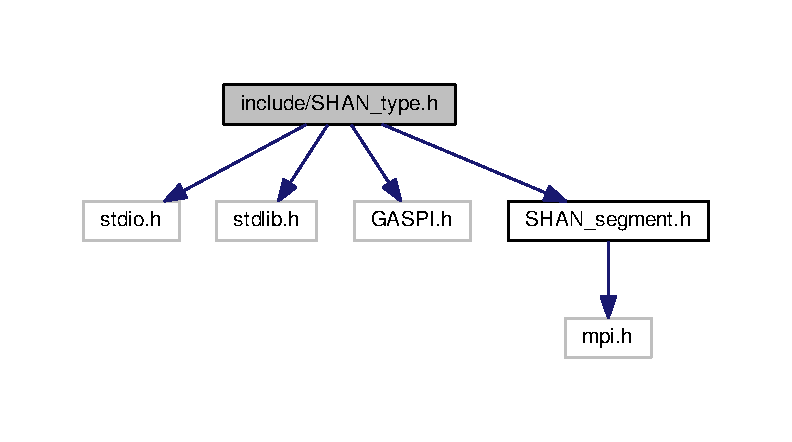
\includegraphics[width=350pt]{SHAN__type_8h__incl}
\end{center}
\end{figure}
\subsection*{Functions}
\begin{DoxyCompactItemize}
\item 
void \hyperlink{SHAN__type_8h_a319a7a3259b544163e6c72aa0b2f4530}{shan\+\_\+comm\+\_\+get\+\_\+local} (\hyperlink{structshan__neighborhood__t}{shan\+\_\+neighborhood\+\_\+t} $\ast$neighborhood\+\_\+id, \hyperlink{structshan__segment__t}{shan\+\_\+segment\+\_\+t} $\ast$data\+\_\+segment, const int type\+\_\+id, const int idx)
\item 
void \hyperlink{SHAN__type_8h_a9cc180e5b3e9c075498625cd61b16523}{shan\+\_\+comm\+\_\+get\+\_\+remote} (\hyperlink{structshan__neighborhood__t}{shan\+\_\+neighborhood\+\_\+t} $\ast$neighborhood\+\_\+id, \hyperlink{structshan__segment__t}{shan\+\_\+segment\+\_\+t} $\ast$const data\+\_\+segment, int const type\+\_\+id, int const idx)
\item 
int \hyperlink{SHAN__type_8h_ab8732eec39c8355b7f6b420ff147c4d6}{shan\+\_\+get\+\_\+shared\+\_\+type} (\hyperlink{structtype__local__t}{type\+\_\+local\+\_\+t} $\ast$type\+\_\+info, \hyperlink{structshan__neighborhood__t}{shan\+\_\+neighborhood\+\_\+t} $\ast$neighborhood\+\_\+id, int local\+\_\+rank, int num\+\_\+neighbors, int type\+\_\+id)
\item 
int \hyperlink{SHAN__type_8h_affaa110499283abb00fcc8f8c53de742}{shan\+\_\+comm\+\_\+type\+\_\+offset} (\hyperlink{structshan__neighborhood__t}{shan\+\_\+neighborhood\+\_\+t} $\ast$neighborhood\+\_\+id, int type\+\_\+id, int $\ast$$\ast$nelem\+\_\+send, int $\ast$$\ast$nelem\+\_\+recv, int $\ast$$\ast$send\+\_\+sz, int $\ast$$\ast$recv\+\_\+sz, long $\ast$$\ast$send\+\_\+offset, long $\ast$$\ast$recv\+\_\+offset)
\item 
int \hyperlink{SHAN__type_8h_aadc9431cf45a459770d1eb188bfd3c47}{shan\+\_\+comm\+\_\+get\+\_\+type} (\hyperlink{structtype__local__t}{type\+\_\+local\+\_\+t} $\ast$type\+\_\+info, void $\ast$shm\+\_\+ptr, int num\+\_\+neighbors, \hyperlink{structshan__element__t}{shan\+\_\+element\+\_\+t} $\ast$type\+\_\+element)
\end{DoxyCompactItemize}


\subsection{Detailed Description}
S\+H\+A\+N\+\_\+type header. Type conversion in shared memory. 



\subsection{Function Documentation}
\index{S\+H\+A\+N\+\_\+type.\+h@{S\+H\+A\+N\+\_\+type.\+h}!shan\+\_\+comm\+\_\+get\+\_\+local@{shan\+\_\+comm\+\_\+get\+\_\+local}}
\index{shan\+\_\+comm\+\_\+get\+\_\+local@{shan\+\_\+comm\+\_\+get\+\_\+local}!S\+H\+A\+N\+\_\+type.\+h@{S\+H\+A\+N\+\_\+type.\+h}}
\subsubsection[{\texorpdfstring{shan\+\_\+comm\+\_\+get\+\_\+local(shan\+\_\+neighborhood\+\_\+t $\ast$neighborhood\+\_\+id, shan\+\_\+segment\+\_\+t $\ast$data\+\_\+segment, const int type\+\_\+id, const int idx)}{shan_comm_get_local(shan_neighborhood_t *neighborhood_id, shan_segment_t *data_segment, const int type_id, const int idx)}}]{\setlength{\rightskip}{0pt plus 5cm}void shan\+\_\+comm\+\_\+get\+\_\+local (
\begin{DoxyParamCaption}
\item[{{\bf shan\+\_\+neighborhood\+\_\+t} $\ast$}]{neighborhood\+\_\+id, }
\item[{{\bf shan\+\_\+segment\+\_\+t} $\ast$}]{data\+\_\+segment, }
\item[{const int}]{type\+\_\+id, }
\item[{const int}]{idx}
\end{DoxyParamCaption}
)}\hypertarget{SHAN__type_8h_a319a7a3259b544163e6c72aa0b2f4530}{}\label{SHAN__type_8h_a319a7a3259b544163e6c72aa0b2f4530}
Converts shared mem send type in shared mem recv type. Finalizes receive in shared mem.


\begin{DoxyParams}{Parameters}
{\em neighborhood\+\_\+id} & -\/ general neighborhood handle \\
\hline
{\em data\+\_\+segment} & -\/ used data segment \\
\hline
{\em type\+\_\+id} & -\/ used type id \\
\hline
{\em idx} & -\/ rank index in neighborhood\\
\hline
\end{DoxyParams}
\begin{DoxyReturn}{Returns}
S\+H\+A\+N\+\_\+\+C\+O\+M\+M\+\_\+\+S\+U\+C\+C\+E\+SS in case of success, S\+H\+A\+N\+\_\+\+C\+O\+M\+M\+\_\+\+E\+R\+R\+OR in case of error. 
\end{DoxyReturn}
\index{S\+H\+A\+N\+\_\+type.\+h@{S\+H\+A\+N\+\_\+type.\+h}!shan\+\_\+comm\+\_\+get\+\_\+remote@{shan\+\_\+comm\+\_\+get\+\_\+remote}}
\index{shan\+\_\+comm\+\_\+get\+\_\+remote@{shan\+\_\+comm\+\_\+get\+\_\+remote}!S\+H\+A\+N\+\_\+type.\+h@{S\+H\+A\+N\+\_\+type.\+h}}
\subsubsection[{\texorpdfstring{shan\+\_\+comm\+\_\+get\+\_\+remote(shan\+\_\+neighborhood\+\_\+t $\ast$neighborhood\+\_\+id, shan\+\_\+segment\+\_\+t $\ast$const data\+\_\+segment, int const type\+\_\+id, int const idx)}{shan_comm_get_remote(shan_neighborhood_t *neighborhood_id, shan_segment_t *const data_segment, int const type_id, int const idx)}}]{\setlength{\rightskip}{0pt plus 5cm}void shan\+\_\+comm\+\_\+get\+\_\+remote (
\begin{DoxyParamCaption}
\item[{{\bf shan\+\_\+neighborhood\+\_\+t} $\ast$}]{neighborhood\+\_\+id, }
\item[{{\bf shan\+\_\+segment\+\_\+t} $\ast$const}]{data\+\_\+segment, }
\item[{int const}]{type\+\_\+id, }
\item[{int const}]{idx}
\end{DoxyParamCaption}
)}\hypertarget{SHAN__type_8h_a9cc180e5b3e9c075498625cd61b16523}{}\label{SHAN__type_8h_a9cc180e5b3e9c075498625cd61b16523}
Finalizes receive for remote comm


\begin{DoxyParams}{Parameters}
{\em neighborhood\+\_\+id} & -\/ general neighborhood handle \\
\hline
{\em data\+\_\+segment} & -\/ used data segment \\
\hline
{\em type\+\_\+id} & -\/ used type id \\
\hline
{\em idx} & -\/ rank index in neighborhood\\
\hline
\end{DoxyParams}
\begin{DoxyReturn}{Returns}
S\+H\+A\+N\+\_\+\+C\+O\+M\+M\+\_\+\+S\+U\+C\+C\+E\+SS in case of success, S\+H\+A\+N\+\_\+\+C\+O\+M\+M\+\_\+\+E\+R\+R\+OR in case of error. 
\end{DoxyReturn}
\index{S\+H\+A\+N\+\_\+type.\+h@{S\+H\+A\+N\+\_\+type.\+h}!shan\+\_\+comm\+\_\+get\+\_\+type@{shan\+\_\+comm\+\_\+get\+\_\+type}}
\index{shan\+\_\+comm\+\_\+get\+\_\+type@{shan\+\_\+comm\+\_\+get\+\_\+type}!S\+H\+A\+N\+\_\+type.\+h@{S\+H\+A\+N\+\_\+type.\+h}}
\subsubsection[{\texorpdfstring{shan\+\_\+comm\+\_\+get\+\_\+type(type\+\_\+local\+\_\+t $\ast$type\+\_\+info, void $\ast$shm\+\_\+ptr, int num\+\_\+neighbors, shan\+\_\+element\+\_\+t $\ast$type\+\_\+element)}{shan_comm_get_type(type_local_t *type_info, void *shm_ptr, int num_neighbors, shan_element_t *type_element)}}]{\setlength{\rightskip}{0pt plus 5cm}int shan\+\_\+comm\+\_\+get\+\_\+type (
\begin{DoxyParamCaption}
\item[{{\bf type\+\_\+local\+\_\+t} $\ast$}]{type\+\_\+info, }
\item[{void $\ast$}]{shm\+\_\+ptr, }
\item[{int}]{num\+\_\+neighbors, }
\item[{{\bf shan\+\_\+element\+\_\+t} $\ast$}]{type\+\_\+element}
\end{DoxyParamCaption}
)}\hypertarget{SHAN__type_8h_aadc9431cf45a459770d1eb188bfd3c47}{}\label{SHAN__type_8h_aadc9431cf45a459770d1eb188bfd3c47}
Getter function for type data


\begin{DoxyParams}{Parameters}
{\em type\+\_\+info} & -\/ type data struct (\hyperlink{SHAN__comm_8h}{S\+H\+A\+N\+\_\+comm.\+h}) \\
\hline
{\em shm\+\_\+ptr} & -\/ pointer to shared memory \\
\hline
{\em num\+\_\+neighbors} & -\/ rank local number of neighbors in neighborhood \\
\hline
{\em type\+\_\+element} & -\/ type element\\
\hline
\end{DoxyParams}
\begin{DoxyReturn}{Returns}
S\+H\+A\+N\+\_\+\+C\+O\+M\+M\+\_\+\+S\+U\+C\+C\+E\+SS in case of success, S\+H\+A\+N\+\_\+\+C\+O\+M\+M\+\_\+\+E\+R\+R\+OR in case of error. 
\end{DoxyReturn}
\index{S\+H\+A\+N\+\_\+type.\+h@{S\+H\+A\+N\+\_\+type.\+h}!shan\+\_\+comm\+\_\+type\+\_\+offset@{shan\+\_\+comm\+\_\+type\+\_\+offset}}
\index{shan\+\_\+comm\+\_\+type\+\_\+offset@{shan\+\_\+comm\+\_\+type\+\_\+offset}!S\+H\+A\+N\+\_\+type.\+h@{S\+H\+A\+N\+\_\+type.\+h}}
\subsubsection[{\texorpdfstring{shan\+\_\+comm\+\_\+type\+\_\+offset(shan\+\_\+neighborhood\+\_\+t $\ast$neighborhood\+\_\+id, int type\+\_\+id, int $\ast$$\ast$nelem\+\_\+send, int $\ast$$\ast$nelem\+\_\+recv, int $\ast$$\ast$send\+\_\+sz, int $\ast$$\ast$recv\+\_\+sz, long $\ast$$\ast$send\+\_\+offset, long $\ast$$\ast$recv\+\_\+offset)}{shan_comm_type_offset(shan_neighborhood_t *neighborhood_id, int type_id, int **nelem_send, int **nelem_recv, int **send_sz, int **recv_sz, long **send_offset, long **recv_offset)}}]{\setlength{\rightskip}{0pt plus 5cm}int shan\+\_\+comm\+\_\+type\+\_\+offset (
\begin{DoxyParamCaption}
\item[{{\bf shan\+\_\+neighborhood\+\_\+t} $\ast$}]{neighborhood\+\_\+id, }
\item[{int}]{type\+\_\+id, }
\item[{int $\ast$$\ast$}]{nelem\+\_\+send, }
\item[{int $\ast$$\ast$}]{nelem\+\_\+recv, }
\item[{int $\ast$$\ast$}]{send\+\_\+sz, }
\item[{int $\ast$$\ast$}]{recv\+\_\+sz, }
\item[{long $\ast$$\ast$}]{send\+\_\+offset, }
\item[{long $\ast$$\ast$}]{recv\+\_\+offset}
\end{DoxyParamCaption}
)}\hypertarget{SHAN__type_8h_affaa110499283abb00fcc8f8c53de742}{}\label{SHAN__type_8h_affaa110499283abb00fcc8f8c53de742}
Gets type data structure for node local ranks


\begin{DoxyParams}{Parameters}
{\em neighborhood\+\_\+id} & -\/ general neighborhood handle \\
\hline
{\em type\+\_\+id} & -\/ used type id \\
\hline
{\em nelem\+\_\+send} & -\/ pointer to number of send elements in shared mem \\
\hline
{\em nelem\+\_\+recv} & -\/ pointer to number of recv elements in shared mem \\
\hline
{\em send\+\_\+sz} & -\/ pointer to send size in shared mem \\
\hline
{\em recv\+\_\+sz} & -\/ pointer to recv size in shared mem \\
\hline
{\em send\+\_\+offset} & -\/ pointer to offset of send elements in shared mem \\
\hline
{\em recv\+\_\+offset} & -\/ pointer to offset of recv elements in shared mem\\
\hline
\end{DoxyParams}
\begin{DoxyReturn}{Returns}
S\+H\+A\+N\+\_\+\+C\+O\+M\+M\+\_\+\+S\+U\+C\+C\+E\+SS in case of success, S\+H\+A\+N\+\_\+\+C\+O\+M\+M\+\_\+\+E\+R\+R\+OR in case of error. 
\end{DoxyReturn}
\index{S\+H\+A\+N\+\_\+type.\+h@{S\+H\+A\+N\+\_\+type.\+h}!shan\+\_\+get\+\_\+shared\+\_\+type@{shan\+\_\+get\+\_\+shared\+\_\+type}}
\index{shan\+\_\+get\+\_\+shared\+\_\+type@{shan\+\_\+get\+\_\+shared\+\_\+type}!S\+H\+A\+N\+\_\+type.\+h@{S\+H\+A\+N\+\_\+type.\+h}}
\subsubsection[{\texorpdfstring{shan\+\_\+get\+\_\+shared\+\_\+type(type\+\_\+local\+\_\+t $\ast$type\+\_\+info, shan\+\_\+neighborhood\+\_\+t $\ast$neighborhood\+\_\+id, int local\+\_\+rank, int num\+\_\+neighbors, int type\+\_\+id)}{shan_get_shared_type(type_local_t *type_info, shan_neighborhood_t *neighborhood_id, int local_rank, int num_neighbors, int type_id)}}]{\setlength{\rightskip}{0pt plus 5cm}int shan\+\_\+get\+\_\+shared\+\_\+type (
\begin{DoxyParamCaption}
\item[{{\bf type\+\_\+local\+\_\+t} $\ast$}]{type\+\_\+info, }
\item[{{\bf shan\+\_\+neighborhood\+\_\+t} $\ast$}]{neighborhood\+\_\+id, }
\item[{int}]{local\+\_\+rank, }
\item[{int}]{num\+\_\+neighbors, }
\item[{int}]{type\+\_\+id}
\end{DoxyParamCaption}
)}\hypertarget{SHAN__type_8h_ab8732eec39c8355b7f6b420ff147c4d6}{}\label{SHAN__type_8h_ab8732eec39c8355b7f6b420ff147c4d6}
Returns type data structure for node local ranks


\begin{DoxyParams}{Parameters}
{\em type\+\_\+info} & -\/ type data struct (\hyperlink{SHAN__comm_8h}{S\+H\+A\+N\+\_\+comm.\+h}) \\
\hline
{\em neighborhood\+\_\+id} & -\/ general neighborhood handle \\
\hline
{\em local\+\_\+rank} & -\/ node local rank \\
\hline
{\em num\+\_\+neighbors} & -\/ number of neighbors \\
\hline
{\em type\+\_\+id} & -\/ used type id\\
\hline
\end{DoxyParams}
\begin{DoxyReturn}{Returns}
S\+H\+A\+N\+\_\+\+C\+O\+M\+M\+\_\+\+S\+U\+C\+C\+E\+SS in case of success, S\+H\+A\+N\+\_\+\+C\+O\+M\+M\+\_\+\+E\+R\+R\+OR in case of error. 
\end{DoxyReturn}

%--- End generated contents ---

% Index
\backmatter
\newpage
\phantomsection
\clearemptydoublepage
\addcontentsline{toc}{chapter}{Index}
\printindex

\end{document}
